\documentclass[1p]{elsarticle_modified}
%\bibliographystyle{elsarticle-num}

%\usepackage[colorlinks]{hyperref}
%\usepackage{abbrmath_seonhwa} %\Abb, \Ascr, \Acal ,\Abf, \Afrak
\usepackage{amsfonts}
\usepackage{amssymb}
\usepackage{amsmath}
\usepackage{amsthm}
\usepackage{scalefnt}
\usepackage{amsbsy}
\usepackage{kotex}
\usepackage{caption}
\usepackage{subfig}
\usepackage{color}
\usepackage{graphicx}
\usepackage{xcolor} %% white, black, red, green, blue, cyan, magenta, yellow
\usepackage{float}
\usepackage{setspace}
\usepackage{hyperref}

\usepackage{tikz}
\usetikzlibrary{arrows}

\usepackage{multirow}
\usepackage{array} % fixed length table
\usepackage{hhline}

%%%%%%%%%%%%%%%%%%%%%
\makeatletter
\renewcommand*\env@matrix[1][\arraystretch]{%
	\edef\arraystretch{#1}%
	\hskip -\arraycolsep
	\let\@ifnextchar\new@ifnextchar
	\array{*\c@MaxMatrixCols c}}
\makeatother %https://tex.stackexchange.com/questions/14071/how-can-i-increase-the-line-spacing-in-a-matrix
%%%%%%%%%%%%%%%

\usepackage[normalem]{ulem}

\newcommand{\msout}[1]{\ifmmode\text{\sout{\ensuremath{#1}}}\else\sout{#1}\fi}
%SOURCE: \msout is \stkout macro in https://tex.stackexchange.com/questions/20609/strikeout-in-math-mode

\newcommand{\cancel}[1]{
	\ifmmode
	{\color{red}\msout{#1}}
	\else
	{\color{red}\sout{#1}}
	\fi
}

\newcommand{\add}[1]{
	{\color{blue}\uwave{#1}}
}

\newcommand{\replace}[2]{
	\ifmmode
	{\color{red}\msout{#1}}{\color{blue}\uwave{#2}}
	\else
	{\color{red}\sout{#1}}{\color{blue}\uwave{#2}}
	\fi
}

\newcommand{\Sol}{\mathcal{S}} %segment
\newcommand{\D}{D} %diagram
\newcommand{\A}{\mathcal{A}} %arc


%%%%%%%%%%%%%%%%%%%%%%%%%%%%%5 test

\def\sl{\operatorname{\textup{SL}}(2,\Cbb)}
\def\psl{\operatorname{\textup{PSL}}(2,\Cbb)}
\def\quan{\mkern 1mu \triangleright \mkern 1mu}

\theoremstyle{definition}
\newtheorem{thm}{Theorem}[section]
\newtheorem{prop}[thm]{Proposition}
\newtheorem{lem}[thm]{Lemma}
\newtheorem{ques}[thm]{Question}
\newtheorem{cor}[thm]{Corollary}
\newtheorem{defn}[thm]{Definition}
\newtheorem{exam}[thm]{Example}
\newtheorem{rmk}[thm]{Remark}
\newtheorem{alg}[thm]{Algorithm}

\newcommand{\I}{\sqrt{-1}}
\begin{document}

%\begin{frontmatter}
%
%\title{Boundary parabolic representations of knots up to 8 crossings}
%
%%% Group authors per affiliation:
%\author{Yunhi Cho} 
%\address{Department of Mathematics, University of Seoul, Seoul, Korea}
%\ead{yhcho@uos.ac.kr}
%
%
%\author{Seonhwa Kim} %\fnref{s_kim}}
%\address{Center for Geometry and Physics, Institute for Basic Science, Pohang, 37673, Korea}
%\ead{ryeona17@ibs.re.kr}
%
%\author{Hyuk Kim}
%\address{Department of Mathematical Sciences, Seoul National University, Seoul 08826, Korea}
%\ead{hyukkim@snu.ac.kr}
%
%\author{Seokbeom Yoon}
%\address{Department of Mathematical Sciences, Seoul National University, Seoul, 08826,  Korea}
%\ead{sbyoon15@snu.ac.kr}
%
%\begin{abstract}
%We find all boundary parabolic representation of knots up to 8 crossings.
%
%\end{abstract}
%\begin{keyword}
%    \MSC[2010] 57M25 
%\end{keyword}
%
%\end{frontmatter}

%\linenumbers
%\tableofcontents
%
\newcommand\colored[1]{\textcolor{white}{\rule[-0.35ex]{0.8em}{1.4ex}}\kern-0.8em\color{red} #1}%
%\newcommand\colored[1]{\textcolor{white}{ #1}\kern-2.17ex	\textcolor{white}{ #1}\kern-1.81ex	\textcolor{white}{ #1}\kern-2.15ex\color{red}#1	}

{\Large $\underline{12a_{0615}~(K12a_{0615})}$}

\setlength{\tabcolsep}{10pt}
\renewcommand{\arraystretch}{1.6}
\vspace{1cm}\begin{tabular}{m{100pt}>{\centering\arraybackslash}m{274pt}}
\multirow{5}{120pt}{
	\centering
	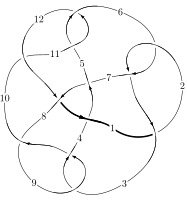
\includegraphics[width=112pt]{../../../GIT/diagram.site/Diagrams/png/1416_12a_0615.png}\\
\ \ \ A knot diagram\footnotemark}&
\allowdisplaybreaks
\textbf{Linearized knot diagam} \\
\cline{2-2}
 &
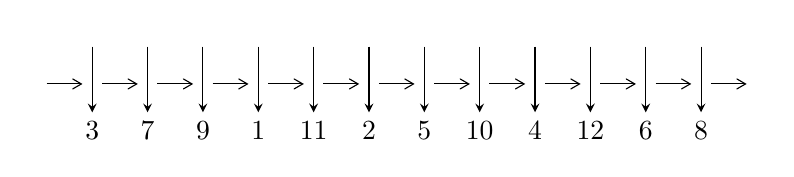
\begin{tikzpicture}[x=20pt, y=17pt]
	% nodes
	\node (C0) at (0, 0) {};
	\node (C1) at (1, 0) {};
	\node (C1U) at (1, +1) {};
	\node (C1D) at (1, -1) {3};

	\node (C2) at (2, 0) {};
	\node (C2U) at (2, +1) {};
	\node (C2D) at (2, -1) {7};

	\node (C3) at (3, 0) {};
	\node (C3U) at (3, +1) {};
	\node (C3D) at (3, -1) {9};

	\node (C4) at (4, 0) {};
	\node (C4U) at (4, +1) {};
	\node (C4D) at (4, -1) {1};

	\node (C5) at (5, 0) {};
	\node (C5U) at (5, +1) {};
	\node (C5D) at (5, -1) {11};

	\node (C6) at (6, 0) {};
	\node (C6U) at (6, +1) {};
	\node (C6D) at (6, -1) {2};

	\node (C7) at (7, 0) {};
	\node (C7U) at (7, +1) {};
	\node (C7D) at (7, -1) {5};

	\node (C8) at (8, 0) {};
	\node (C8U) at (8, +1) {};
	\node (C8D) at (8, -1) {10};

	\node (C9) at (9, 0) {};
	\node (C9U) at (9, +1) {};
	\node (C9D) at (9, -1) {4};

	\node (C10) at (10, 0) {};
	\node (C10U) at (10, +1) {};
	\node (C10D) at (10, -1) {12};

	\node (C11) at (11, 0) {};
	\node (C11U) at (11, +1) {};
	\node (C11D) at (11, -1) {6};

	\node (C12) at (12, 0) {};
	\node (C12U) at (12, +1) {};
	\node (C12D) at (12, -1) {8};
	\node (C13) at (13, 0) {};

	% arrows
	\draw[->,>={angle 60}]
	(C0) edge (C1) (C1) edge (C2) (C2) edge (C3) (C3) edge (C4) (C4) edge (C5) (C5) edge (C6) (C6) edge (C7) (C7) edge (C8) (C8) edge (C9) (C9) edge (C10) (C10) edge (C11) (C11) edge (C12) (C12) edge (C13) ;	\draw[->,>=stealth]
	(C1U) edge (C1D) (C2U) edge (C2D) (C3U) edge (C3D) (C4U) edge (C4D) (C5U) edge (C5D) (C6U) edge (C6D) (C7U) edge (C7D) (C8U) edge (C8D) (C9U) edge (C9D) (C10U) edge (C10D) (C11U) edge (C11D) (C12U) edge (C12D) ;
	\end{tikzpicture} \\
\hhline{~~} \\& 
\textbf{Solving Sequence} \\ \cline{2-2} 
 &
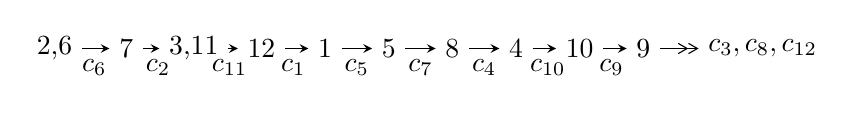
\begin{tikzpicture}[x=23pt, y=7pt]
	% node
	\node (A0) at (-1/8, 0) {2,6};
	\node (A1) at (1, 0) {7};
	\node (A2) at (33/16, 0) {3,11};
	\node (A3) at (25/8, 0) {12};
	\node (A4) at (33/8, 0) {1};
	\node (A5) at (41/8, 0) {5};
	\node (A6) at (49/8, 0) {8};
	\node (A7) at (57/8, 0) {4};
	\node (A8) at (65/8, 0) {10};
	\node (A9) at (73/8, 0) {9};
	\node (C1) at (1/2, -1) {$c_{6}$};
	\node (C2) at (3/2, -1) {$c_{2}$};
	\node (C3) at (21/8, -1) {$c_{11}$};
	\node (C4) at (29/8, -1) {$c_{1}$};
	\node (C5) at (37/8, -1) {$c_{5}$};
	\node (C6) at (45/8, -1) {$c_{7}$};
	\node (C7) at (53/8, -1) {$c_{4}$};
	\node (C8) at (61/8, -1) {$c_{10}$};
	\node (C9) at (69/8, -1) {$c_{9}$};
	\node (A10) at (11, 0) {$c_{3},c_{8},c_{12}$};

	% edge
	\draw[->,>=stealth]	
	(A0) edge (A1) (A1) edge (A2) (A2) edge (A3) (A3) edge (A4) (A4) edge (A5) (A5) edge (A6) (A6) edge (A7) (A7) edge (A8) (A8) edge (A9) ;
	\draw[->>,>={angle 60}]	
	(A9) edge (A10);
\end{tikzpicture} \\ 

\end{tabular} \\

\footnotetext{
The image of knot diagram is generated by the software ``\textbf{Draw programme}" developed by Andrew Bartholomew(\url{http://www.layer8.co.uk/maths/draw/index.htm\#Running-draw}), where we modified some parts for our purpose(\url{https://github.com/CATsTAILs/LinksPainter}).
}\phantom \\ \newline 
\centering \textbf{Ideals for irreducible components\footnotemark of $X_{\text{par}}$} 
 
\begin{align*}
I^u_{1}&=\langle 
b- u,\;u^5+u^4-2 u^2+a- u,\;u^7+u^6- u^5-3 u^4+2 u^2+2 u-1\rangle \\
I^u_{2}&=\langle 
b- u,\;3 u^{21}+2 u^{20}+\cdots+2 a+6,\;u^{22}-3 u^{21}+\cdots-2 u+1\rangle \\
I^u_{3}&=\langle 
- u^{21}+4 u^{20}+\cdots+2 b+3,\;-5 u^{21}+14 u^{20}+\cdots+2 a+7,\;u^{22}-3 u^{21}+\cdots-2 u+1\rangle \\
I^u_{4}&=\langle 
-2489 u^{21}-8939 u^{20}+\cdots+2212 b-39100,\;8695 u^{21}+75565 u^{20}+\cdots+4424 a-81736,\\
\phantom{I^u_{4}}&\phantom{= \langle  }u^{22}+9 u^{21}+\cdots-8 u-8\rangle \\
I^u_{5}&=\langle 
b+u,\;- u^5+u^4+a- u+2,\;u^7- u^6- u^5+u^4+2 u^3-2 u^2+1\rangle \\
I^u_{6}&=\langle 
-708 u^{35} a+2695 u^{35}+\cdots+9336 a+5225,\;708 u^{35} a+584 u^{35}+\cdots-348 a-950,\\
\phantom{I^u_{6}}&\phantom{= \langle  }u^{36}-3 u^{35}+\cdots-4 u+3\rangle \\
I^u_{7}&=\langle 
b+u,\;- u^6+2 u^4- u^3-3 u^2+a+2 u+1,\;u^7+u^6- u^5- u^4+2 u^3+u^2- u-1\rangle \\
I^u_{8}&=\langle 
- u^6- u^5+u^4+u^3-2 u^2+b- u+1,\;- u^6- u^5-2 u^2+a- u,\;u^7+u^6- u^5- u^4+2 u^3+u^2- u-1\rangle \\
I^u_{9}&=\langle 
u^6- u^5- u^4+2 u^3+u^2+b- u-1,\;u^6- u^5- u^4+u^3+2 u^2+a- u-2,\;u^7- u^6- u^5+2 u^4+u^3- u^2- u+1\rangle \\
I^u_{10}&=\langle 
b,\;a+1,\;u+1\rangle \\
\end{align*}\\
\begin{align*}
I^u_{11}&=\langle 
b+1,\;a+2,\;u+1\rangle \\
I^u_{12}&=\langle 
b+1,\;a+3,\;u+1\rangle \\
\\
I^v_{1}&=\langle 
a,\;b+1,\;v-1\rangle \\
\end{align*}
\raggedright * 13 irreducible components of $\dim_{\mathbb{C}}=0$, with total 177 representations.\\
\footnotetext{All coefficients of polynomials are rational numbers. But the coefficients are sometimes approximated in decimal forms when there is not enough margin.}
\newpage
\renewcommand{\arraystretch}{1}
\centering \section*{I. $I^u_{1}= \langle b- u,\;u^5+u^4-2 u^2+a- u,\;u^7+u^6- u^5-3 u^4+2 u^2+2 u-1 \rangle$}
\flushleft \textbf{(i) Arc colorings}\\
\begin{tabular}{m{7pt} m{180pt} m{7pt} m{180pt} }
\flushright $a_{2}=$&$\begin{pmatrix}0\\u\end{pmatrix}$ \\
\flushright $a_{6}=$&$\begin{pmatrix}1\\0\end{pmatrix}$ \\
\flushright $a_{7}=$&$\begin{pmatrix}1\\u^2\end{pmatrix}$ \\
\flushright $a_{3}=$&$\begin{pmatrix}- u\\- u^3+u\end{pmatrix}$ \\
\flushright $a_{11}=$&$\begin{pmatrix}- u^5- u^4+2 u^2+u\\u\end{pmatrix}$ \\
\flushright $a_{12}=$&$\begin{pmatrix}- u^5- u^4+2 u^2\\u\end{pmatrix}$ \\
\flushright $a_{1}=$&$\begin{pmatrix}u^3\\u^5- u^3+u\end{pmatrix}$ \\
\flushright $a_{5}=$&$\begin{pmatrix}u^6+u^5-2 u^3- u^2+1\\- u^2\end{pmatrix}$ \\
\flushright $a_{8}=$&$\begin{pmatrix}u^6+u^5- u^3- u^2+1\\u^5- u^3- u^2+u\end{pmatrix}$ \\
\flushright $a_{4}=$&$\begin{pmatrix}u^5+u^4-2 u^2+1\\u^2- u\end{pmatrix}$ \\
\flushright $a_{10}=$&$\begin{pmatrix}- u+1\\- u^3+u\end{pmatrix}$ \\
\flushright $a_{9}=$&$\begin{pmatrix}u^6+u^5-2 u^3+1\\- u^2+u\end{pmatrix}$\\&\end{tabular}
\flushleft \textbf{(ii) Obstruction class $= -1$}\\~\\
\flushleft \textbf{(iii) Cusp Shapes $= 6 u^4+3 u^3-3 u^2-12 u-12$}\\~\\
\newpage\renewcommand{\arraystretch}{1}
\flushleft \textbf{(iv) u-Polynomials at the component}\newline \\
\begin{tabular}{m{50pt}|m{274pt}}
Crossings & \hspace{64pt}u-Polynomials at each crossing \\
\hline $$\begin{aligned}c_{1},c_{8},c_{10}\end{aligned}$$&$\begin{aligned}
&u^7+3 u^6+7 u^5+9 u^4+10 u^3+10 u^2+8 u+1
\end{aligned}$\\
\hline $$\begin{aligned}c_{2},c_{3},c_{5}\\c_{6},c_{9},c_{11}\end{aligned}$$&$\begin{aligned}
&u^7- u^6- u^5+3 u^4-2 u^2+2 u+1
\end{aligned}$\\
\hline $$\begin{aligned}c_{4},c_{7},c_{12}\end{aligned}$$&$\begin{aligned}
&u^7-6 u^6+18 u^5-32 u^4+35 u^3-21 u^2+3 u+3
\end{aligned}$\\
\hline
\end{tabular}\\~\\
\newpage\renewcommand{\arraystretch}{1}
\flushleft \textbf{(v) Riley Polynomials at the component}\newline \\
\begin{tabular}{m{50pt}|m{274pt}}
Crossings & \hspace{64pt}Riley Polynomials at each crossing \\
\hline $$\begin{aligned}c_{1},c_{8},c_{10}\end{aligned}$$&$\begin{aligned}
&y^7+5 y^6+15 y^5+15 y^4+26 y^3+42 y^2+44 y-1
\end{aligned}$\\
\hline $$\begin{aligned}c_{2},c_{3},c_{5}\\c_{6},c_{9},c_{11}\end{aligned}$$&$\begin{aligned}
&y^7-3 y^6+7 y^5-9 y^4+10 y^3-10 y^2+8 y-1
\end{aligned}$\\
\hline $$\begin{aligned}c_{4},c_{7},c_{12}\end{aligned}$$&$\begin{aligned}
&y^7+10 y^5-10 y^4+25 y^3-39 y^2+135 y-9
\end{aligned}$\\
\hline
\end{tabular}\\~\\
\newpage\flushleft \textbf{(vi) Complex Volumes and Cusp Shapes}
$$\begin{array}{c|c|c}  
\text{Solutions to }I^u_{1}& \I (\text{vol} + \sqrt{-1}CS) & \text{Cusp shape}\\
 \hline 
\begin{aligned}
u &= -0.627087 + 0.878886 I \\
a &= -0.251298 - 0.695933 I \\
b &= -0.627087 + 0.878886 I\end{aligned}
 & \phantom{-}7.19181 - 1.70769 I & -6.14495 - 1.15014 I \\ \hline\begin{aligned}
u &= -0.627087 - 0.878886 I \\
a &= -0.251298 + 0.695933 I \\
b &= -0.627087 - 0.878886 I\end{aligned}
 & \phantom{-}7.19181 + 1.70769 I & -6.14495 + 1.15014 I \\ \hline\begin{aligned}
u &= \phantom{-}1.066700 + 0.299026 I \\
a &= \phantom{-}2.13291 - 1.39668 I \\
b &= \phantom{-}1.066700 + 0.299026 I\end{aligned}
 & -7.70407 - 2.73497 I & -21.0094 + 5.5060 I \\ \hline\begin{aligned}
u &= \phantom{-}1.066700 - 0.299026 I \\
a &= \phantom{-}2.13291 + 1.39668 I \\
b &= \phantom{-}1.066700 - 0.299026 I\end{aligned}
 & -7.70407 + 2.73497 I & -21.0094 - 5.5060 I \\ \hline\begin{aligned}
u &= -1.132720 + 0.725853 I \\
a &= -1.70846 - 1.34533 I \\
b &= -1.132720 + 0.725853 I\end{aligned}
 & \phantom{-}2.4536 + 19.8535 I & -12.4578 - 11.4641 I \\ \hline\begin{aligned}
u &= -1.132720 - 0.725853 I \\
a &= -1.70846 + 1.34533 I \\
b &= -1.132720 - 0.725853 I\end{aligned}
 & \phantom{-}2.4536 - 19.8535 I & -12.4578 + 11.4641 I \\ \hline\begin{aligned}
u &= \phantom{-}0.386210\phantom{ +0.000000I} \\
a &= \phantom{-}0.653686\phantom{ +0.000000I} \\
b &= \phantom{-}0.386210\phantom{ +0.000000I}\end{aligned}
 & -0.592790\phantom{ +0.000000I} & -16.7760\phantom{ +0.000000I}\\
 \hline 
 \end{array}$$\newpage\newpage\renewcommand{\arraystretch}{1}
\centering \section*{II. $I^u_{2}= \langle b- u,\;3 u^{21}+2 u^{20}+\cdots+2 a+6,\;u^{22}-3 u^{21}+\cdots-2 u+1 \rangle$}
\flushleft \textbf{(i) Arc colorings}\\
\begin{tabular}{m{7pt} m{180pt} m{7pt} m{180pt} }
\flushright $a_{2}=$&$\begin{pmatrix}0\\u\end{pmatrix}$ \\
\flushright $a_{6}=$&$\begin{pmatrix}1\\0\end{pmatrix}$ \\
\flushright $a_{7}=$&$\begin{pmatrix}1\\u^2\end{pmatrix}$ \\
\flushright $a_{3}=$&$\begin{pmatrix}- u\\- u^3+u\end{pmatrix}$ \\
\flushright $a_{11}=$&$\begin{pmatrix}-\frac{3}{2} u^{21}- u^{20}+\cdots+\frac{9}{2} u-3\\u\end{pmatrix}$ \\
\flushright $a_{12}=$&$\begin{pmatrix}-\frac{3}{2} u^{21}- u^{20}+\cdots+\frac{7}{2} u-3\\u\end{pmatrix}$ \\
\flushright $a_{1}=$&$\begin{pmatrix}u^3\\u^5- u^3+u\end{pmatrix}$ \\
\flushright $a_{5}=$&$\begin{pmatrix}\frac{11}{2} u^{21}-8 u^{20}+\cdots+6 u-\frac{1}{2}\\- u^2\end{pmatrix}$ \\
\flushright $a_{8}=$&$\begin{pmatrix}\frac{41}{2} u^{21}-\frac{65}{2} u^{20}+\cdots+\frac{43}{2} u-\frac{13}{2}\\-\frac{1}{2} u^{21}-\frac{11}{2} u^{20}+\cdots+2 u-5\end{pmatrix}$ \\
\flushright $a_{4}=$&$\begin{pmatrix}3 u^{21}-6 u^{20}+\cdots+4 u-1\\-\frac{3}{2} u^{21}+\frac{9}{2} u^{20}+\cdots-\frac{5}{2} u+\frac{5}{2}\end{pmatrix}$ \\
\flushright $a_{10}=$&$\begin{pmatrix}7 u^{21}-\frac{37}{2} u^{20}+\cdots+14 u-\frac{17}{2}\\- u^3+u\end{pmatrix}$ \\
\flushright $a_{9}=$&$\begin{pmatrix}\frac{1}{2} u^{21}- u^{20}+\cdots+\frac{5}{2} u-1\\\frac{3}{2} u^{21}-\frac{9}{2} u^{20}+\cdots+\frac{5}{2} u-\frac{5}{2}\end{pmatrix}$\\&\end{tabular}
\flushleft \textbf{(ii) Obstruction class $= -1$}\\~\\
\flushleft \textbf{(iii) Cusp Shapes $= 6 u^{21}-22 u^{20}-3 u^{19}+83 u^{18}-38 u^{17}-188 u^{16}+170 u^{15}+255 u^{14}-367 u^{13}-200 u^{12}+523 u^{11}+42 u^{10}-531 u^9+145 u^8+346 u^7-200 u^6-136 u^5+138 u^4-53 u^2+20 u-23$}\\~\\
\newpage\renewcommand{\arraystretch}{1}
\flushleft \textbf{(iv) u-Polynomials at the component}\newline \\
\begin{tabular}{m{50pt}|m{274pt}}
Crossings & \hspace{64pt}u-Polynomials at each crossing \\
\hline $$\begin{aligned}c_{1},c_{10}\end{aligned}$$&$\begin{aligned}
&u^{22}+9 u^{21}+\cdots-6 u+1
\end{aligned}$\\
\hline $$\begin{aligned}c_{2},c_{5},c_{6}\\c_{11}\end{aligned}$$&$\begin{aligned}
&u^{22}+3 u^{21}+\cdots+2 u+1
\end{aligned}$\\
\hline $$\begin{aligned}c_{3},c_{9}\end{aligned}$$&$\begin{aligned}
&u^{22}-9 u^{21}+\cdots+8 u-8
\end{aligned}$\\
\hline $$\begin{aligned}c_{4},c_{12}\end{aligned}$$&$\begin{aligned}
&u^{22}+4 u^{21}+\cdots+4 u+1
\end{aligned}$\\
\hline $$\begin{aligned}c_{7}\end{aligned}$$&$\begin{aligned}
&u^{22}-24 u^{21}+\cdots-53248 u+4096
\end{aligned}$\\
\hline $$\begin{aligned}c_{8}\end{aligned}$$&$\begin{aligned}
&u^{22}+7 u^{21}+\cdots+2528 u+64
\end{aligned}$\\
\hline
\end{tabular}\\~\\
\newpage\renewcommand{\arraystretch}{1}
\flushleft \textbf{(v) Riley Polynomials at the component}\newline \\
\begin{tabular}{m{50pt}|m{274pt}}
Crossings & \hspace{64pt}Riley Polynomials at each crossing \\
\hline $$\begin{aligned}c_{1},c_{10}\end{aligned}$$&$\begin{aligned}
&y^{22}+11 y^{21}+\cdots-54 y+1
\end{aligned}$\\
\hline $$\begin{aligned}c_{2},c_{5},c_{6}\\c_{11}\end{aligned}$$&$\begin{aligned}
&y^{22}-9 y^{21}+\cdots+6 y+1
\end{aligned}$\\
\hline $$\begin{aligned}c_{3},c_{9}\end{aligned}$$&$\begin{aligned}
&y^{22}-7 y^{21}+\cdots-2528 y+64
\end{aligned}$\\
\hline $$\begin{aligned}c_{4},c_{12}\end{aligned}$$&$\begin{aligned}
&y^{22}+6 y^{21}+\cdots+2 y+1
\end{aligned}$\\
\hline $$\begin{aligned}c_{7}\end{aligned}$$&$\begin{aligned}
&y^{22}+70 y^{20}+\cdots-159383552 y+16777216
\end{aligned}$\\
\hline $$\begin{aligned}c_{8}\end{aligned}$$&$\begin{aligned}
&y^{22}+13 y^{21}+\cdots-5071360 y+4096
\end{aligned}$\\
\hline
\end{tabular}\\~\\
\newpage\flushleft \textbf{(vi) Complex Volumes and Cusp Shapes}
$$\begin{array}{c|c|c}  
\text{Solutions to }I^u_{2}& \I (\text{vol} + \sqrt{-1}CS) & \text{Cusp shape}\\
 \hline 
\begin{aligned}
u &= -0.836840 + 0.581799 I \\
a &= -1.72055 - 3.05333 I \\
b &= -0.836840 + 0.581799 I\end{aligned}
 & \phantom{-}2.49482 - 0.03580 I & -9.19656 - 1.18782 I \\ \hline\begin{aligned}
u &= -0.836840 - 0.581799 I \\
a &= -1.72055 + 3.05333 I \\
b &= -0.836840 - 0.581799 I\end{aligned}
 & \phantom{-}2.49482 + 0.03580 I & -9.19656 + 1.18782 I \\ \hline\begin{aligned}
u &= -0.958571\phantom{ +0.000000I} \\
a &= -3.30128\phantom{ +0.000000I} \\
b &= -0.958571\phantom{ +0.000000I}\end{aligned}
 & -4.93723\phantom{ +0.000000I} & -17.9860\phantom{ +0.000000I} \\ \hline\begin{aligned}
u &= -0.795188 + 0.673491 I \\
a &= \phantom{-}0.482964 - 1.043980 I \\
b &= -0.795188 + 0.673491 I\end{aligned}
 & \phantom{-}4.79008 + 3.04512 I & -1.46454 - 3.95630 I \\ \hline\begin{aligned}
u &= -0.795188 - 0.673491 I \\
a &= \phantom{-}0.482964 + 1.043980 I \\
b &= -0.795188 - 0.673491 I\end{aligned}
 & \phantom{-}4.79008 - 3.04512 I & -1.46454 + 3.95630 I \\ \hline\begin{aligned}
u &= -1.08445\phantom{ +0.000000I} \\
a &= -2.31049\phantom{ +0.000000I} \\
b &= -1.08445\phantom{ +0.000000I}\end{aligned}
 & -5.01957\phantom{ +0.000000I} & -16.9370\phantom{ +0.000000I} \\ \hline\begin{aligned}
u &= \phantom{-}0.580710 + 0.919219 I \\
a &= \phantom{-}0.325305 - 0.694106 I \\
b &= \phantom{-}0.580710 + 0.919219 I\end{aligned}
 & \phantom{-}5.86563 + 7.62274 I & -8.03926 - 3.67301 I \\ \hline\begin{aligned}
u &= \phantom{-}0.580710 - 0.919219 I \\
a &= \phantom{-}0.325305 + 0.694106 I \\
b &= \phantom{-}0.580710 - 0.919219 I\end{aligned}
 & \phantom{-}5.86563 - 7.62274 I & -8.03926 + 3.67301 I \\ \hline\begin{aligned}
u &= \phantom{-}0.919954 + 0.624468 I \\
a &= \phantom{-}2.09163 - 2.53678 I \\
b &= \phantom{-}0.919954 + 0.624468 I\end{aligned}
 & \phantom{-}4.00179 - 7.08200 I & -5.03530 + 8.12849 I \\ \hline\begin{aligned}
u &= \phantom{-}0.919954 - 0.624468 I \\
a &= \phantom{-}2.09163 + 2.53678 I \\
b &= \phantom{-}0.919954 - 0.624468 I\end{aligned}
 & \phantom{-}4.00179 + 7.08200 I & -5.03530 - 8.12849 I\\
 \hline 
 \end{array}$$\newpage$$\begin{array}{c|c|c}  
\text{Solutions to }I^u_{2}& \I (\text{vol} + \sqrt{-1}CS) & \text{Cusp shape}\\
 \hline 
\begin{aligned}
u &= \phantom{-}0.906778 + 0.649704 I \\
a &= -0.03604 - 1.82735 I \\
b &= \phantom{-}0.906778 + 0.649704 I\end{aligned}
 & \phantom{-}2.00908 - 9.79924 I & -10.3132 + 13.5800 I \\ \hline\begin{aligned}
u &= \phantom{-}0.906778 - 0.649704 I \\
a &= -0.03604 + 1.82735 I \\
b &= \phantom{-}0.906778 - 0.649704 I\end{aligned}
 & \phantom{-}2.00908 + 9.79924 I & -10.3132 - 13.5800 I \\ \hline\begin{aligned}
u &= \phantom{-}0.514242 + 0.653281 I \\
a &= \phantom{-}0.268297 - 0.175648 I \\
b &= \phantom{-}0.514242 + 0.653281 I\end{aligned}
 & -0.046256 + 1.148600 I & -11.80195 - 1.32419 I \\ \hline\begin{aligned}
u &= \phantom{-}0.514242 - 0.653281 I \\
a &= \phantom{-}0.268297 + 0.175648 I \\
b &= \phantom{-}0.514242 - 0.653281 I\end{aligned}
 & -0.046256 - 1.148600 I & -11.80195 + 1.32419 I \\ \hline\begin{aligned}
u &= \phantom{-}1.201870 + 0.120067 I \\
a &= \phantom{-}2.05957 - 0.60124 I \\
b &= \phantom{-}1.201870 + 0.120067 I\end{aligned}
 & -6.50144 + 3.58049 I & -19.3843 - 4.8932 I \\ \hline\begin{aligned}
u &= \phantom{-}1.201870 - 0.120067 I \\
a &= \phantom{-}2.05957 + 0.60124 I \\
b &= \phantom{-}1.201870 - 0.120067 I\end{aligned}
 & -6.50144 - 3.58049 I & -19.3843 + 4.8932 I \\ \hline\begin{aligned}
u &= -1.073910 + 0.601774 I \\
a &= -2.29187 - 1.39130 I \\
b &= -1.073910 + 0.601774 I\end{aligned}
 & -3.37508 + 11.10700 I & -16.0470 - 11.0853 I \\ \hline\begin{aligned}
u &= -1.073910 - 0.601774 I \\
a &= -2.29187 + 1.39130 I \\
b &= -1.073910 - 0.601774 I\end{aligned}
 & -3.37508 - 11.10700 I & -16.0470 + 11.0853 I \\ \hline\begin{aligned}
u &= \phantom{-}1.093640 + 0.715729 I \\
a &= \phantom{-}1.76706 - 1.47100 I \\
b &= \phantom{-}1.093640 + 0.715729 I\end{aligned}
 & \phantom{-}4.2815 - 13.6348 I & -10.24905 + 7.91781 I \\ \hline\begin{aligned}
u &= \phantom{-}1.093640 - 0.715729 I \\
a &= \phantom{-}1.76706 + 1.47100 I \\
b &= \phantom{-}1.093640 - 0.715729 I\end{aligned}
 & \phantom{-}4.2815 + 13.6348 I & -10.24905 - 7.91781 I\\
 \hline 
 \end{array}$$\newpage$$\begin{array}{c|c|c}  
\text{Solutions to }I^u_{2}& \I (\text{vol} + \sqrt{-1}CS) & \text{Cusp shape}\\
 \hline 
\begin{aligned}
u &= \phantom{-}0.010269 + 0.423690 I \\
a &= \phantom{-}0.85952 + 2.24965 I \\
b &= \phantom{-}0.010269 + 0.423690 I\end{aligned}
 & \phantom{-}2.15030 - 2.68120 I & -8.00708 + 4.43159 I \\ \hline\begin{aligned}
u &= \phantom{-}0.010269 - 0.423690 I \\
a &= \phantom{-}0.85952 - 2.24965 I \\
b &= \phantom{-}0.010269 - 0.423690 I\end{aligned}
 & \phantom{-}2.15030 + 2.68120 I & -8.00708 - 4.43159 I\\
 \hline 
 \end{array}$$\newpage\newpage\renewcommand{\arraystretch}{1}
\centering \section*{III. $I^u_{3}= \langle - u^{21}+4 u^{20}+\cdots+2 b+3,\;-5 u^{21}+14 u^{20}+\cdots+2 a+7,\;u^{22}-3 u^{21}+\cdots-2 u+1 \rangle$}
\flushleft \textbf{(i) Arc colorings}\\
\begin{tabular}{m{7pt} m{180pt} m{7pt} m{180pt} }
\flushright $a_{2}=$&$\begin{pmatrix}0\\u\end{pmatrix}$ \\
\flushright $a_{6}=$&$\begin{pmatrix}1\\0\end{pmatrix}$ \\
\flushright $a_{7}=$&$\begin{pmatrix}1\\u^2\end{pmatrix}$ \\
\flushright $a_{3}=$&$\begin{pmatrix}- u\\- u^3+u\end{pmatrix}$ \\
\flushright $a_{11}=$&$\begin{pmatrix}\frac{5}{2} u^{21}-7 u^{20}+\cdots+6 u-\frac{7}{2}\\\frac{1}{2} u^{21}-2 u^{20}+\cdots-3 u^2-\frac{3}{2}\end{pmatrix}$ \\
\flushright $a_{12}=$&$\begin{pmatrix}2 u^{21}-5 u^{20}+\cdots+6 u-2\\\frac{1}{2} u^{21}-2 u^{20}+\cdots-3 u^2-\frac{3}{2}\end{pmatrix}$ \\
\flushright $a_{1}=$&$\begin{pmatrix}u^3\\u^5- u^3+u\end{pmatrix}$ \\
\flushright $a_{5}=$&$\begin{pmatrix}\frac{3}{2} u^{21}-8 u^{20}+\cdots+\frac{11}{2} u-5\\-4 u^{21}+6 u^{20}+\cdots-\frac{11}{2} u+\frac{1}{2}\end{pmatrix}$ \\
\flushright $a_{8}=$&$\begin{pmatrix}-3 u^{21}+\frac{11}{2} u^{20}+\cdots-\frac{7}{2} u+3\\3 u^{20}-\frac{7}{2} u^{19}+\cdots-\frac{1}{2} u+\frac{3}{2}\end{pmatrix}$ \\
\flushright $a_{4}=$&$\begin{pmatrix}\frac{17}{2} u^{21}-\frac{35}{2} u^{20}+\cdots+\frac{23}{2} u-\frac{11}{2}\\-\frac{7}{2} u^{21}+2 u^{20}+\cdots-3 u-\frac{5}{2}\end{pmatrix}$ \\
\flushright $a_{10}=$&$\begin{pmatrix}-\frac{5}{2} u^{21}+11 u^{20}+\cdots-\frac{11}{2} u+8\\11 u^{21}-\frac{49}{2} u^{20}+\cdots+15 u-\frac{21}{2}\end{pmatrix}$ \\
\flushright $a_{9}=$&$\begin{pmatrix}\frac{11}{2} u^{21}-8 u^{20}+\cdots+6 u-\frac{1}{2}\\\frac{5}{2} u^{21}-11 u^{20}+\cdots+\frac{11}{2} u-7\end{pmatrix}$\\&\end{tabular}
\flushleft \textbf{(ii) Obstruction class $= -1$}\\~\\
\flushleft \textbf{(iii) Cusp Shapes $= 6 u^{21}-22 u^{20}-3 u^{19}+83 u^{18}-38 u^{17}-188 u^{16}+170 u^{15}+255 u^{14}-367 u^{13}-200 u^{12}+523 u^{11}+42 u^{10}-531 u^9+145 u^8+346 u^7-200 u^6-136 u^5+138 u^4-53 u^2+20 u-23$}\\~\\
\newpage\renewcommand{\arraystretch}{1}
\flushleft \textbf{(iv) u-Polynomials at the component}\newline \\
\begin{tabular}{m{50pt}|m{274pt}}
Crossings & \hspace{64pt}u-Polynomials at each crossing \\
\hline $$\begin{aligned}c_{1},c_{8}\end{aligned}$$&$\begin{aligned}
&u^{22}+9 u^{21}+\cdots-6 u+1
\end{aligned}$\\
\hline $$\begin{aligned}c_{2},c_{3},c_{6}\\c_{9}\end{aligned}$$&$\begin{aligned}
&u^{22}+3 u^{21}+\cdots+2 u+1
\end{aligned}$\\
\hline $$\begin{aligned}c_{4}\end{aligned}$$&$\begin{aligned}
&u^{22}-24 u^{21}+\cdots-53248 u+4096
\end{aligned}$\\
\hline $$\begin{aligned}c_{5},c_{11}\end{aligned}$$&$\begin{aligned}
&u^{22}-9 u^{21}+\cdots+8 u-8
\end{aligned}$\\
\hline $$\begin{aligned}c_{7},c_{12}\end{aligned}$$&$\begin{aligned}
&u^{22}+4 u^{21}+\cdots+4 u+1
\end{aligned}$\\
\hline $$\begin{aligned}c_{10}\end{aligned}$$&$\begin{aligned}
&u^{22}+7 u^{21}+\cdots+2528 u+64
\end{aligned}$\\
\hline
\end{tabular}\\~\\
\newpage\renewcommand{\arraystretch}{1}
\flushleft \textbf{(v) Riley Polynomials at the component}\newline \\
\begin{tabular}{m{50pt}|m{274pt}}
Crossings & \hspace{64pt}Riley Polynomials at each crossing \\
\hline $$\begin{aligned}c_{1},c_{8}\end{aligned}$$&$\begin{aligned}
&y^{22}+11 y^{21}+\cdots-54 y+1
\end{aligned}$\\
\hline $$\begin{aligned}c_{2},c_{3},c_{6}\\c_{9}\end{aligned}$$&$\begin{aligned}
&y^{22}-9 y^{21}+\cdots+6 y+1
\end{aligned}$\\
\hline $$\begin{aligned}c_{4}\end{aligned}$$&$\begin{aligned}
&y^{22}+70 y^{20}+\cdots-159383552 y+16777216
\end{aligned}$\\
\hline $$\begin{aligned}c_{5},c_{11}\end{aligned}$$&$\begin{aligned}
&y^{22}-7 y^{21}+\cdots-2528 y+64
\end{aligned}$\\
\hline $$\begin{aligned}c_{7},c_{12}\end{aligned}$$&$\begin{aligned}
&y^{22}+6 y^{21}+\cdots+2 y+1
\end{aligned}$\\
\hline $$\begin{aligned}c_{10}\end{aligned}$$&$\begin{aligned}
&y^{22}+13 y^{21}+\cdots-5071360 y+4096
\end{aligned}$\\
\hline
\end{tabular}\\~\\
\newpage\flushleft \textbf{(vi) Complex Volumes and Cusp Shapes}
$$\begin{array}{c|c|c}  
\text{Solutions to }I^u_{3}& \I (\text{vol} + \sqrt{-1}CS) & \text{Cusp shape}\\
 \hline 
\begin{aligned}
u &= -0.836840 + 0.581799 I \\
a &= -0.079524 - 0.136665 I \\
b &= -1.101550 - 0.880614 I\end{aligned}
 & \phantom{-}2.49482 - 0.03580 I & -9.19656 - 1.18782 I \\ \hline\begin{aligned}
u &= -0.836840 - 0.581799 I \\
a &= -0.079524 + 0.136665 I \\
b &= -1.101550 + 0.880614 I\end{aligned}
 & \phantom{-}2.49482 + 0.03580 I & -9.19656 + 1.18782 I \\ \hline\begin{aligned}
u &= -0.958571\phantom{ +0.000000I} \\
a &= -1.05475\phantom{ +0.000000I} \\
b &= \phantom{-}0.168704\phantom{ +0.000000I}\end{aligned}
 & -4.93723\phantom{ +0.000000I} & -17.9860\phantom{ +0.000000I} \\ \hline\begin{aligned}
u &= -0.795188 + 0.673491 I \\
a &= \phantom{-}0.892746 - 0.143126 I \\
b &= -0.302170 - 1.111950 I\end{aligned}
 & \phantom{-}4.79008 + 3.04512 I & -1.46454 - 3.95630 I \\ \hline\begin{aligned}
u &= -0.795188 - 0.673491 I \\
a &= \phantom{-}0.892746 + 0.143126 I \\
b &= -0.302170 + 1.111950 I\end{aligned}
 & \phantom{-}4.79008 - 3.04512 I & -1.46454 + 3.95630 I \\ \hline\begin{aligned}
u &= -1.08445\phantom{ +0.000000I} \\
a &= -1.47024\phantom{ +0.000000I} \\
b &= -0.658865\phantom{ +0.000000I}\end{aligned}
 & -5.01957\phantom{ +0.000000I} & -16.9370\phantom{ +0.000000I} \\ \hline\begin{aligned}
u &= \phantom{-}0.580710 + 0.919219 I \\
a &= -0.476892 - 0.652029 I \\
b &= -1.057640 + 0.718065 I\end{aligned}
 & \phantom{-}5.86563 + 7.62274 I & -8.03926 - 3.67301 I \\ \hline\begin{aligned}
u &= \phantom{-}0.580710 - 0.919219 I \\
a &= -0.476892 + 0.652029 I \\
b &= -1.057640 - 0.718065 I\end{aligned}
 & \phantom{-}5.86563 - 7.62274 I & -8.03926 + 3.67301 I \\ \hline\begin{aligned}
u &= \phantom{-}0.919954 + 0.624468 I \\
a &= -0.930867 + 0.453984 I \\
b &= -0.599409 - 1.137210 I\end{aligned}
 & \phantom{-}4.00179 - 7.08200 I & -5.03530 + 8.12849 I \\ \hline\begin{aligned}
u &= \phantom{-}0.919954 - 0.624468 I \\
a &= -0.930867 - 0.453984 I \\
b &= -0.599409 + 1.137210 I\end{aligned}
 & \phantom{-}4.00179 + 7.08200 I & -5.03530 - 8.12849 I\\
 \hline 
 \end{array}$$\newpage$$\begin{array}{c|c|c}  
\text{Solutions to }I^u_{3}& \I (\text{vol} + \sqrt{-1}CS) & \text{Cusp shape}\\
 \hline 
\begin{aligned}
u &= \phantom{-}0.906778 + 0.649704 I \\
a &= -1.70529 + 1.50502 I \\
b &= -1.24193 - 0.77433 I\end{aligned}
 & \phantom{-}2.00908 - 9.79924 I & -10.3132 + 13.5800 I \\ \hline\begin{aligned}
u &= \phantom{-}0.906778 - 0.649704 I \\
a &= -1.70529 - 1.50502 I \\
b &= -1.24193 + 0.77433 I\end{aligned}
 & \phantom{-}2.00908 + 9.79924 I & -10.3132 - 13.5800 I \\ \hline\begin{aligned}
u &= \phantom{-}0.514242 + 0.653281 I \\
a &= \phantom{-}0.769810 - 0.437698 I \\
b &= \phantom{-}1.090770 - 0.240404 I\end{aligned}
 & -0.046256 + 1.148600 I & -11.80195 - 1.32419 I \\ \hline\begin{aligned}
u &= \phantom{-}0.514242 - 0.653281 I \\
a &= \phantom{-}0.769810 + 0.437698 I \\
b &= \phantom{-}1.090770 + 0.240404 I\end{aligned}
 & -0.046256 - 1.148600 I & -11.80195 + 1.32419 I \\ \hline\begin{aligned}
u &= \phantom{-}1.201870 + 0.120067 I \\
a &= -2.05250 + 0.39422 I \\
b &= -0.998510 + 0.502784 I\end{aligned}
 & -6.50144 + 3.58049 I & -19.3843 - 4.8932 I \\ \hline\begin{aligned}
u &= \phantom{-}1.201870 - 0.120067 I \\
a &= -2.05250 - 0.39422 I \\
b &= -0.998510 - 0.502784 I\end{aligned}
 & -6.50144 - 3.58049 I & -19.3843 + 4.8932 I \\ \hline\begin{aligned}
u &= -1.073910 + 0.601774 I \\
a &= \phantom{-}1.72007 + 0.95190 I \\
b &= \phantom{-}1.375940 - 0.121987 I\end{aligned}
 & -3.37508 + 11.10700 I & -16.0470 - 11.0853 I \\ \hline\begin{aligned}
u &= -1.073910 - 0.601774 I \\
a &= \phantom{-}1.72007 - 0.95190 I \\
b &= \phantom{-}1.375940 + 0.121987 I\end{aligned}
 & -3.37508 - 11.10700 I & -16.0470 + 11.0853 I \\ \hline\begin{aligned}
u &= \phantom{-}1.093640 + 0.715729 I \\
a &= \phantom{-}0.513238 + 0.359274 I \\
b &= -0.545268 + 0.984025 I\end{aligned}
 & \phantom{-}4.2815 - 13.6348 I & -10.24905 + 7.91781 I \\ \hline\begin{aligned}
u &= \phantom{-}1.093640 - 0.715729 I \\
a &= \phantom{-}0.513238 - 0.359274 I \\
b &= -0.545268 - 0.984025 I\end{aligned}
 & \phantom{-}4.2815 + 13.6348 I & -10.24905 - 7.91781 I\\
 \hline 
 \end{array}$$\newpage$$\begin{array}{c|c|c}  
\text{Solutions to }I^u_{3}& \I (\text{vol} + \sqrt{-1}CS) & \text{Cusp shape}\\
 \hline 
\begin{aligned}
u &= \phantom{-}0.010269 + 0.423690 I \\
a &= \phantom{-}0.111698 + 1.290160 I \\
b &= -0.875150 - 0.696689 I\end{aligned}
 & \phantom{-}2.15030 - 2.68120 I & -8.00708 + 4.43159 I \\ \hline\begin{aligned}
u &= \phantom{-}0.010269 - 0.423690 I \\
a &= \phantom{-}0.111698 - 1.290160 I \\
b &= -0.875150 + 0.696689 I\end{aligned}
 & \phantom{-}2.15030 + 2.68120 I & -8.00708 - 4.43159 I\\
 \hline 
 \end{array}$$\newpage\newpage\renewcommand{\arraystretch}{1}
\centering \section*{IV. $I^u_{4}= \langle -2489 u^{21}-8939 u^{20}+\cdots+2212 b-39100,\;8695 u^{21}+75565 u^{20}+\cdots+4424 a-81736,\;u^{22}+9 u^{21}+\cdots-8 u-8 \rangle$}
\flushleft \textbf{(i) Arc colorings}\\
\begin{tabular}{m{7pt} m{180pt} m{7pt} m{180pt} }
\flushright $a_{2}=$&$\begin{pmatrix}0\\u\end{pmatrix}$ \\
\flushright $a_{6}=$&$\begin{pmatrix}1\\0\end{pmatrix}$ \\
\flushright $a_{7}=$&$\begin{pmatrix}1\\u^2\end{pmatrix}$ \\
\flushright $a_{3}=$&$\begin{pmatrix}- u\\- u^3+u\end{pmatrix}$ \\
\flushright $a_{11}=$&$\begin{pmatrix}-1.96542 u^{21}-17.0807 u^{20}+\cdots+21.8454 u+18.4756\\1.12523 u^{21}+4.04114 u^{20}+\cdots-10.3834 u+17.6763\end{pmatrix}$ \\
\flushright $a_{12}=$&$\begin{pmatrix}-3.09064 u^{21}-21.1218 u^{20}+\cdots+32.2288 u+0.799277\\1.12523 u^{21}+4.04114 u^{20}+\cdots-10.3834 u+17.6763\end{pmatrix}$ \\
\flushright $a_{1}=$&$\begin{pmatrix}u^3\\u^5- u^3+u\end{pmatrix}$ \\
\flushright $a_{5}=$&$\begin{pmatrix}6.31736 u^{21}+53.0095 u^{20}+\cdots+15.0077 u-55.9593\\2.25723 u^{21}+22.5665 u^{20}+\cdots+5.23237 u-40.3580\end{pmatrix}$ \\
\flushright $a_{8}=$&$\begin{pmatrix}-4.21090 u^{21}-33.7579 u^{20}+\cdots-3.57188 u+20.5018\\-0.244123 u^{21}-3.93038 u^{20}+\cdots+1.53255 u+10.5841\end{pmatrix}$ \\
\flushright $a_{4}=$&$\begin{pmatrix}-1.05335 u^{21}-4.45886 u^{20}+\cdots+27.7238 u-13.1094\\-1.97604 u^{21}-16.8892 u^{20}+\cdots+14.8635 u+7.68897\end{pmatrix}$ \\
\flushright $a_{10}=$&$\begin{pmatrix}-4.06533 u^{21}-34.7642 u^{20}+\cdots+14.0420 u+27.5461\\5.82188 u^{21}+44.0823 u^{20}+\cdots-22.9096 u-17.9331\end{pmatrix}$ \\
\flushright $a_{9}=$&$\begin{pmatrix}-4.48440 u^{21}-31.0364 u^{20}+\cdots+2.54792 u-3.33454\\-4.63608 u^{21}-42.5158 u^{20}+\cdots+14.7848 u+49.8608\end{pmatrix}$\\&\end{tabular}
\flushleft \textbf{(ii) Obstruction class $= -1$}\\~\\
\flushleft \textbf{(iii) Cusp Shapes $= -\frac{223}{553} u^{21}+\frac{601}{79} u^{20}+\cdots+\frac{44196}{553} u-\frac{62234}{553}$}\\~\\
\newpage\renewcommand{\arraystretch}{1}
\flushleft \textbf{(iv) u-Polynomials at the component}\newline \\
\begin{tabular}{m{50pt}|m{274pt}}
Crossings & \hspace{64pt}u-Polynomials at each crossing \\
\hline $$\begin{aligned}c_{1}\end{aligned}$$&$\begin{aligned}
&u^{22}+7 u^{21}+\cdots+2528 u+64
\end{aligned}$\\
\hline $$\begin{aligned}c_{2},c_{6}\end{aligned}$$&$\begin{aligned}
&u^{22}-9 u^{21}+\cdots+8 u-8
\end{aligned}$\\
\hline $$\begin{aligned}c_{3},c_{5},c_{9}\\c_{11}\end{aligned}$$&$\begin{aligned}
&u^{22}+3 u^{21}+\cdots+2 u+1
\end{aligned}$\\
\hline $$\begin{aligned}c_{4},c_{7}\end{aligned}$$&$\begin{aligned}
&u^{22}+4 u^{21}+\cdots+4 u+1
\end{aligned}$\\
\hline $$\begin{aligned}c_{8},c_{10}\end{aligned}$$&$\begin{aligned}
&u^{22}+9 u^{21}+\cdots-6 u+1
\end{aligned}$\\
\hline $$\begin{aligned}c_{12}\end{aligned}$$&$\begin{aligned}
&u^{22}-24 u^{21}+\cdots-53248 u+4096
\end{aligned}$\\
\hline
\end{tabular}\\~\\
\newpage\renewcommand{\arraystretch}{1}
\flushleft \textbf{(v) Riley Polynomials at the component}\newline \\
\begin{tabular}{m{50pt}|m{274pt}}
Crossings & \hspace{64pt}Riley Polynomials at each crossing \\
\hline $$\begin{aligned}c_{1}\end{aligned}$$&$\begin{aligned}
&y^{22}+13 y^{21}+\cdots-5071360 y+4096
\end{aligned}$\\
\hline $$\begin{aligned}c_{2},c_{6}\end{aligned}$$&$\begin{aligned}
&y^{22}-7 y^{21}+\cdots-2528 y+64
\end{aligned}$\\
\hline $$\begin{aligned}c_{3},c_{5},c_{9}\\c_{11}\end{aligned}$$&$\begin{aligned}
&y^{22}-9 y^{21}+\cdots+6 y+1
\end{aligned}$\\
\hline $$\begin{aligned}c_{4},c_{7}\end{aligned}$$&$\begin{aligned}
&y^{22}+6 y^{21}+\cdots+2 y+1
\end{aligned}$\\
\hline $$\begin{aligned}c_{8},c_{10}\end{aligned}$$&$\begin{aligned}
&y^{22}+11 y^{21}+\cdots-54 y+1
\end{aligned}$\\
\hline $$\begin{aligned}c_{12}\end{aligned}$$&$\begin{aligned}
&y^{22}+70 y^{20}+\cdots-159383552 y+16777216
\end{aligned}$\\
\hline
\end{tabular}\\~\\
\newpage\flushleft \textbf{(vi) Complex Volumes and Cusp Shapes}
$$\begin{array}{c|c|c}  
\text{Solutions to }I^u_{4}& \I (\text{vol} + \sqrt{-1}CS) & \text{Cusp shape}\\
 \hline 
\begin{aligned}
u &= \phantom{-}1.090770 + 0.240404 I \\
a &= \phantom{-}0.542580 - 0.374285 I \\
b &= \phantom{-}0.514242 - 0.653281 I\end{aligned}
 & -0.046256 - 1.148600 I & -11.80195 + 1.32419 I \\ \hline\begin{aligned}
u &= \phantom{-}1.090770 - 0.240404 I \\
a &= \phantom{-}0.542580 + 0.374285 I \\
b &= \phantom{-}0.514242 + 0.653281 I\end{aligned}
 & -0.046256 + 1.148600 I & -11.80195 - 1.32419 I \\ \hline\begin{aligned}
u &= -0.998510 + 0.502784 I \\
a &= \phantom{-}2.10010 + 0.82977 I \\
b &= \phantom{-}1.201870 + 0.120067 I\end{aligned}
 & -6.50144 + 3.58049 I & -19.3843 - 4.8932 I \\ \hline\begin{aligned}
u &= -0.998510 - 0.502784 I \\
a &= \phantom{-}2.10010 - 0.82977 I \\
b &= \phantom{-}1.201870 - 0.120067 I\end{aligned}
 & -6.50144 - 3.58049 I & -19.3843 + 4.8932 I \\ \hline\begin{aligned}
u &= -0.875150 + 0.696689 I \\
a &= \phantom{-}0.347791 + 0.346084 I \\
b &= \phantom{-}0.010269 - 0.423690 I\end{aligned}
 & \phantom{-}2.15030 + 2.68120 I & -8.00708 - 4.43159 I \\ \hline\begin{aligned}
u &= -0.875150 - 0.696689 I \\
a &= \phantom{-}0.347791 - 0.346084 I \\
b &= \phantom{-}0.010269 + 0.423690 I\end{aligned}
 & \phantom{-}2.15030 - 2.68120 I & -8.00708 + 4.43159 I \\ \hline\begin{aligned}
u &= -0.545268 + 0.984025 I \\
a &= \phantom{-}0.460061 - 0.564019 I \\
b &= \phantom{-}1.093640 + 0.715729 I\end{aligned}
 & \phantom{-}4.2815 - 13.6348 I & -10.24905 + 7.91781 I \\ \hline\begin{aligned}
u &= -0.545268 - 0.984025 I \\
a &= \phantom{-}0.460061 + 0.564019 I \\
b &= \phantom{-}1.093640 - 0.715729 I\end{aligned}
 & \phantom{-}4.2815 + 13.6348 I & -10.24905 - 7.91781 I \\ \hline\begin{aligned}
u &= -0.302170 + 1.111950 I \\
a &= -0.459228 + 0.676532 I \\
b &= -0.795188 - 0.673491 I\end{aligned}
 & \phantom{-}4.79008 - 3.04512 I & -1.46454 + 3.95630 I \\ \hline\begin{aligned}
u &= -0.302170 - 1.111950 I \\
a &= -0.459228 - 0.676532 I \\
b &= -0.795188 + 0.673491 I\end{aligned}
 & \phantom{-}4.79008 + 3.04512 I & -1.46454 - 3.95630 I\\
 \hline 
 \end{array}$$\newpage$$\begin{array}{c|c|c}  
\text{Solutions to }I^u_{4}& \I (\text{vol} + \sqrt{-1}CS) & \text{Cusp shape}\\
 \hline 
\begin{aligned}
u &= -1.057640 + 0.718065 I \\
a &= -0.567651 + 0.387084 I \\
b &= \phantom{-}0.580710 + 0.919219 I\end{aligned}
 & \phantom{-}5.86563 + 7.62274 I & -8.03926 - 3.67301 I \\ \hline\begin{aligned}
u &= -1.057640 - 0.718065 I \\
a &= -0.567651 - 0.387084 I \\
b &= \phantom{-}0.580710 - 0.919219 I\end{aligned}
 & \phantom{-}5.86563 - 7.62274 I & -8.03926 + 3.67301 I \\ \hline\begin{aligned}
u &= -0.599409 + 1.137210 I \\
a &= \phantom{-}0.526068 + 0.725042 I \\
b &= \phantom{-}0.919954 - 0.624468 I\end{aligned}
 & \phantom{-}4.00179 + 7.08200 I & -5.03530 - 8.12849 I \\ \hline\begin{aligned}
u &= -0.599409 - 1.137210 I \\
a &= \phantom{-}0.526068 - 0.725042 I \\
b &= \phantom{-}0.919954 + 0.624468 I\end{aligned}
 & \phantom{-}4.00179 - 7.08200 I & -5.03530 + 8.12849 I \\ \hline\begin{aligned}
u &= -0.658865\phantom{ +0.000000I} \\
a &= -2.41993\phantom{ +0.000000I} \\
b &= -1.08445\phantom{ +0.000000I}\end{aligned}
 & -5.01957\phantom{ +0.000000I} & -16.9370\phantom{ +0.000000I} \\ \hline\begin{aligned}
u &= \phantom{-}1.375940 + 0.121987 I \\
a &= -1.74592 + 0.14546 I \\
b &= -1.073910 - 0.601774 I\end{aligned}
 & -3.37508 - 11.10700 I & -16.0470 + 11.0853 I \\ \hline\begin{aligned}
u &= \phantom{-}1.375940 - 0.121987 I \\
a &= -1.74592 - 0.14546 I \\
b &= -1.073910 + 0.601774 I\end{aligned}
 & -3.37508 + 11.10700 I & -16.0470 - 11.0853 I \\ \hline\begin{aligned}
u &= -1.101550 + 0.880614 I \\
a &= -0.1110480 - 0.0269532 I \\
b &= -0.836840 - 0.581799 I\end{aligned}
 & \phantom{-}2.49482 + 0.03580 I & -9.19656 + 1.18782 I \\ \hline\begin{aligned}
u &= -1.101550 - 0.880614 I \\
a &= -0.1110480 + 0.0269532 I \\
b &= -0.836840 + 0.581799 I\end{aligned}
 & \phantom{-}2.49482 - 0.03580 I & -9.19656 - 1.18782 I \\ \hline\begin{aligned}
u &= -1.24193 + 0.77433 I \\
a &= \phantom{-}1.37068 + 1.06137 I \\
b &= \phantom{-}0.906778 - 0.649704 I\end{aligned}
 & \phantom{-}2.00908 + 9.79924 I & -10.3132 - 13.5800 I\\
 \hline 
 \end{array}$$\newpage$$\begin{array}{c|c|c}  
\text{Solutions to }I^u_{4}& \I (\text{vol} + \sqrt{-1}CS) & \text{Cusp shape}\\
 \hline 
\begin{aligned}
u &= -1.24193 - 0.77433 I \\
a &= \phantom{-}1.37068 - 1.06137 I \\
b &= \phantom{-}0.906778 + 0.649704 I\end{aligned}
 & \phantom{-}2.00908 - 9.79924 I & -10.3132 + 13.5800 I \\ \hline\begin{aligned}
u &= \phantom{-}0.168704\phantom{ +0.000000I} \\
a &= \phantom{-}5.99308\phantom{ +0.000000I} \\
b &= -0.958571\phantom{ +0.000000I}\end{aligned}
 & -4.93723\phantom{ +0.000000I} & -17.9860\phantom{ +0.000000I}\\
 \hline 
 \end{array}$$\newpage\newpage\renewcommand{\arraystretch}{1}
\centering \section*{V. $I^u_{5}= \langle b+u,\;- u^5+u^4+a- u+2,\;u^7- u^6- u^5+u^4+2 u^3-2 u^2+1 \rangle$}
\flushleft \textbf{(i) Arc colorings}\\
\begin{tabular}{m{7pt} m{180pt} m{7pt} m{180pt} }
\flushright $a_{2}=$&$\begin{pmatrix}0\\u\end{pmatrix}$ \\
\flushright $a_{6}=$&$\begin{pmatrix}1\\0\end{pmatrix}$ \\
\flushright $a_{7}=$&$\begin{pmatrix}1\\u^2\end{pmatrix}$ \\
\flushright $a_{3}=$&$\begin{pmatrix}- u\\- u^3+u\end{pmatrix}$ \\
\flushright $a_{11}=$&$\begin{pmatrix}u^5- u^4+u-2\\- u\end{pmatrix}$ \\
\flushright $a_{12}=$&$\begin{pmatrix}u^5- u^4+2 u-2\\- u\end{pmatrix}$ \\
\flushright $a_{1}=$&$\begin{pmatrix}u^3\\u^5- u^3+u\end{pmatrix}$ \\
\flushright $a_{5}=$&$\begin{pmatrix}u^6- u^5+u^2-2 u+1\\- u^2\end{pmatrix}$ \\
\flushright $a_{8}=$&$\begin{pmatrix}- u^6+u^5- u^3- u^2+2 u-1\\- u^5+u^3+u^2- u\end{pmatrix}$ \\
\flushright $a_{4}=$&$\begin{pmatrix}- u^5+u^4-2 u+1\\- u^2+u\end{pmatrix}$ \\
\flushright $a_{10}=$&$\begin{pmatrix}u-1\\u^3- u\end{pmatrix}$ \\
\flushright $a_{9}=$&$\begin{pmatrix}- u^6+u^5-2 u^2+2 u-1\\u^2- u\end{pmatrix}$\\&\end{tabular}
\flushleft \textbf{(ii) Obstruction class $= 1$}\\~\\
\flushleft \textbf{(iii) Cusp Shapes $= 6 u^6-6 u^4-3 u^3+15 u^2-12$}\\~\\
\newpage\renewcommand{\arraystretch}{1}
\flushleft \textbf{(iv) u-Polynomials at the component}\newline \\
\begin{tabular}{m{50pt}|m{274pt}}
Crossings & \hspace{64pt}u-Polynomials at each crossing \\
\hline $$\begin{aligned}c_{1},c_{8},c_{10}\end{aligned}$$&$\begin{aligned}
&u^7-3 u^6+7 u^5-9 u^4+10 u^3-6 u^2+4 u-1
\end{aligned}$\\
\hline $$\begin{aligned}c_{2},c_{5},c_{9}\end{aligned}$$&$\begin{aligned}
&u^7+u^6- u^5- u^4+2 u^3+2 u^2-1
\end{aligned}$\\
\hline $$\begin{aligned}c_{3},c_{6},c_{11}\end{aligned}$$&$\begin{aligned}
&u^7- u^6- u^5+u^4+2 u^3-2 u^2+1
\end{aligned}$\\
\hline $$\begin{aligned}c_{4},c_{7},c_{12}\end{aligned}$$&$\begin{aligned}
&u^7- u^3+u^2- u+1
\end{aligned}$\\
\hline
\end{tabular}\\~\\
\newpage\renewcommand{\arraystretch}{1}
\flushleft \textbf{(v) Riley Polynomials at the component}\newline \\
\begin{tabular}{m{50pt}|m{274pt}}
Crossings & \hspace{64pt}Riley Polynomials at each crossing \\
\hline $$\begin{aligned}c_{1},c_{8},c_{10}\end{aligned}$$&$\begin{aligned}
&y^7+5 y^6+15 y^5+31 y^4+42 y^3+26 y^2+4 y-1
\end{aligned}$\\
\hline $$\begin{aligned}c_{2},c_{3},c_{5}\\c_{6},c_{9},c_{11}\end{aligned}$$&$\begin{aligned}
&y^7-3 y^6+7 y^5-9 y^4+10 y^3-6 y^2+4 y-1
\end{aligned}$\\
\hline $$\begin{aligned}c_{4},c_{7},c_{12}\end{aligned}$$&$\begin{aligned}
&y^7-2 y^5-2 y^4+y^3+y^2- y-1
\end{aligned}$\\
\hline
\end{tabular}\\~\\
\newpage\flushleft \textbf{(vi) Complex Volumes and Cusp Shapes}
$$\begin{array}{c|c|c}  
\text{Solutions to }I^u_{5}& \I (\text{vol} + \sqrt{-1}CS) & \text{Cusp shape}\\
 \hline 
\begin{aligned}
u &= \phantom{-}0.624311 + 0.652659 I \\
a &= -1.088180 + 0.242247 I \\
b &= -0.624311 - 0.652659 I\end{aligned}
 & \phantom{-}3.14416 - 4.35714 I & -6.47040 + 7.89451 I \\ \hline\begin{aligned}
u &= \phantom{-}0.624311 - 0.652659 I \\
a &= -1.088180 - 0.242247 I \\
b &= -0.624311 + 0.652659 I\end{aligned}
 & \phantom{-}3.14416 + 4.35714 I & -6.47040 - 7.89451 I \\ \hline\begin{aligned}
u &= -0.938309 + 0.714070 I \\
a &= \phantom{-}0.98531 + 1.45468 I \\
b &= \phantom{-}0.938309 - 0.714070 I\end{aligned}
 & \phantom{-}2.23584 + 8.24520 I & -9.99047 - 7.58188 I \\ \hline\begin{aligned}
u &= -0.938309 - 0.714070 I \\
a &= \phantom{-}0.98531 - 1.45468 I \\
b &= \phantom{-}0.938309 + 0.714070 I\end{aligned}
 & \phantom{-}2.23584 - 8.24520 I & -9.99047 + 7.58188 I \\ \hline\begin{aligned}
u &= \phantom{-}1.111470 + 0.496667 I \\
a &= -1.99974 + 0.62011 I \\
b &= -1.111470 - 0.496667 I\end{aligned}
 & -1.76596 - 9.37850 I & -13.2669 + 9.6588 I \\ \hline\begin{aligned}
u &= \phantom{-}1.111470 - 0.496667 I \\
a &= -1.99974 - 0.62011 I \\
b &= -1.111470 + 0.496667 I\end{aligned}
 & -1.76596 + 9.37850 I & -13.2669 - 9.6588 I \\ \hline\begin{aligned}
u &= -0.594946\phantom{ +0.000000I} \\
a &= -2.79477\phantom{ +0.000000I} \\
b &= \phantom{-}0.594946\phantom{ +0.000000I}\end{aligned}
 & -3.93822\phantom{ +0.000000I} & -6.54450\phantom{ +0.000000I}\\
 \hline 
 \end{array}$$\newpage\newpage\renewcommand{\arraystretch}{1}
\centering \section*{VI. $I^u_{6}= \langle -708 u^{35} a+2695 u^{35}+\cdots+9336 a+5225,\;708 u^{35} a+584 u^{35}+\cdots-348 a-950,\;u^{36}-3 u^{35}+\cdots-4 u+3 \rangle$}
\flushleft \textbf{(i) Arc colorings}\\
\begin{tabular}{m{7pt} m{180pt} m{7pt} m{180pt} }
\flushright $a_{2}=$&$\begin{pmatrix}0\\u\end{pmatrix}$ \\
\flushright $a_{6}=$&$\begin{pmatrix}1\\0\end{pmatrix}$ \\
\flushright $a_{7}=$&$\begin{pmatrix}1\\u^2\end{pmatrix}$ \\
\flushright $a_{3}=$&$\begin{pmatrix}- u\\- u^3+u\end{pmatrix}$ \\
\flushright $a_{11}=$&$\begin{pmatrix}a\\0.404110 a u^{35}-1.53824 u^{35}+\cdots-5.32877 a-2.98231\end{pmatrix}$ \\
\flushright $a_{12}=$&$\begin{pmatrix}-0.404110 a u^{35}+1.53824 u^{35}+\cdots+6.32877 a+2.98231\\0.404110 a u^{35}-1.53824 u^{35}+\cdots-5.32877 a-2.98231\end{pmatrix}$ \\
\flushright $a_{1}=$&$\begin{pmatrix}u^3\\u^5- u^3+u\end{pmatrix}$ \\
\flushright $a_{5}=$&$\begin{pmatrix}1.71176 a u^{35}-19.1083 u^{35}+\cdots-18.2323 a+42.1745\\2.54966 a u^{35}-6.68779 u^{35}+\cdots-18.3476 a+31.5645\end{pmatrix}$ \\
\flushright $a_{8}=$&$\begin{pmatrix}17.4024 a u^{35}+15.4395 u^{35}+\cdots-6.81678 a-34.0765\\-7.90240 a u^{35}-16.1895 u^{35}+\cdots+3.56678 a+48.3265\end{pmatrix}$ \\
\flushright $a_{4}=$&$\begin{pmatrix}9.90354 a u^{35}-12.8651 u^{35}+\cdots-23.5748 a-7.02759\\-1.64212 a u^{35}-11.1809 u^{35}+\cdots-16.7551 a+58.0166\end{pmatrix}$ \\
\flushright $a_{10}=$&$\begin{pmatrix}4.29737 a u^{35}+40.7131 u^{35}+\cdots+0.168379 a-110.825\\-0.205479 a u^{35}-34.0879 u^{35}+\cdots-11.0616 a+58.8653\end{pmatrix}$ \\
\flushright $a_{9}=$&$\begin{pmatrix}-0.235160 a u^{35}+21.5818 u^{35}+\cdots+7.64612 a-21.6560\\2.10959 a u^{35}-2.70034 u^{35}+\cdots-7.76712 a-31.8476\end{pmatrix}$\\&\end{tabular}
\flushleft \textbf{(ii) Obstruction class $= -1$}\\~\\
\flushleft \textbf{(iii) Cusp Shapes $= -20 u^{35}+59 u^{34}+68 u^{33}-401 u^{32}+23 u^{31}+1440 u^{30}-896 u^{29}-3434 u^{28}+3778 u^{27}+5817 u^{26}-9944 u^{25}-6644 u^{24}+19472 u^{23}+3275 u^{22}-29861 u^{21}+5436 u^{20}+36810 u^{19}-16946 u^{18}-36863 u^{17}+26081 u^{16}+30326 u^{15}-28140 u^{14}-21370 u^{13}+23633 u^{12}+13830 u^{11}-16213 u^{10}-8829 u^9+9789 u^8+5308 u^7-5435 u^6-2437 u^5+2520 u^4+690 u^3-790 u^2-83 u+105$}\\~\\
\newpage\renewcommand{\arraystretch}{1}
\flushleft \textbf{(iv) u-Polynomials at the component}\newline \\
\begin{tabular}{m{50pt}|m{274pt}}
Crossings & \hspace{64pt}u-Polynomials at each crossing \\
\hline $$\begin{aligned}c_{1},c_{8},c_{10}\end{aligned}$$&$\begin{aligned}
&(u^{36}+13 u^{35}+\cdots+124 u+9)^{2}
\end{aligned}$\\
\hline $$\begin{aligned}c_{2},c_{3},c_{5}\\c_{6},c_{9},c_{11}\end{aligned}$$&$\begin{aligned}
&(u^{36}+3 u^{35}+\cdots+4 u+3)^{2}
\end{aligned}$\\
\hline $$\begin{aligned}c_{4},c_{7},c_{12}\end{aligned}$$&$\begin{aligned}
&(u^{36}+9 u^{35}+\cdots+10 u+1)^{2}
\end{aligned}$\\
\hline
\end{tabular}\\~\\
\newpage\renewcommand{\arraystretch}{1}
\flushleft \textbf{(v) Riley Polynomials at the component}\newline \\
\begin{tabular}{m{50pt}|m{274pt}}
Crossings & \hspace{64pt}Riley Polynomials at each crossing \\
\hline $$\begin{aligned}c_{1},c_{8},c_{10}\end{aligned}$$&$\begin{aligned}
&(y^{36}+23 y^{35}+\cdots+248 y+81)^{2}
\end{aligned}$\\
\hline $$\begin{aligned}c_{2},c_{3},c_{5}\\c_{6},c_{9},c_{11}\end{aligned}$$&$\begin{aligned}
&(y^{36}-13 y^{35}+\cdots-124 y+9)^{2}
\end{aligned}$\\
\hline $$\begin{aligned}c_{4},c_{7},c_{12}\end{aligned}$$&$\begin{aligned}
&(y^{36}+9 y^{35}+\cdots-2 y+1)^{2}
\end{aligned}$\\
\hline
\end{tabular}\\~\\
\newpage\flushleft \textbf{(vi) Complex Volumes and Cusp Shapes}
$$\begin{array}{c|c|c}  
\text{Solutions to }I^u_{6}& \I (\text{vol} + \sqrt{-1}CS) & \text{Cusp shape}\\
 \hline 
\begin{aligned}
u &= \phantom{-}0.765456 + 0.633383 I \\
a &= -0.940028 - 0.378523 I \\
b &= \phantom{-}0.449327 - 1.113840 I\end{aligned}
 & \phantom{-}4.48033 + 2.14866 I & -2.67250 - 1.35700 I \\ \hline\begin{aligned}
u &= \phantom{-}0.765456 + 0.633383 I \\
a &= -0.25382 - 1.52848 I \\
b &= -0.897412 + 0.669456 I\end{aligned}
 & \phantom{-}4.48033 + 2.14866 I & -2.67250 - 1.35700 I \\ \hline\begin{aligned}
u &= \phantom{-}0.765456 - 0.633383 I \\
a &= -0.940028 + 0.378523 I \\
b &= \phantom{-}0.449327 + 1.113840 I\end{aligned}
 & \phantom{-}4.48033 - 2.14866 I & -2.67250 + 1.35700 I \\ \hline\begin{aligned}
u &= \phantom{-}0.765456 - 0.633383 I \\
a &= -0.25382 + 1.52848 I \\
b &= -0.897412 - 0.669456 I\end{aligned}
 & \phantom{-}4.48033 - 2.14866 I & -2.67250 + 1.35700 I \\ \hline\begin{aligned}
u &= \phantom{-}0.791040 + 0.669232 I \\
a &= \phantom{-}1.43100 - 0.12353 I \\
b &= -0.874503 + 0.590035 I\end{aligned}
 & \phantom{-}2.36818 + 4.68398 I & -9.65950 - 6.77168 I \\ \hline\begin{aligned}
u &= \phantom{-}0.791040 + 0.669232 I \\
a &= \phantom{-}0.126481 - 0.130137 I \\
b &= \phantom{-}1.161280 - 0.806628 I\end{aligned}
 & \phantom{-}2.36818 + 4.68398 I & -9.65950 - 6.77168 I \\ \hline\begin{aligned}
u &= \phantom{-}0.791040 - 0.669232 I \\
a &= \phantom{-}1.43100 + 0.12353 I \\
b &= -0.874503 - 0.590035 I\end{aligned}
 & \phantom{-}2.36818 - 4.68398 I & -9.65950 + 6.77168 I \\ \hline\begin{aligned}
u &= \phantom{-}0.791040 - 0.669232 I \\
a &= \phantom{-}0.126481 + 0.130137 I \\
b &= \phantom{-}1.161280 + 0.806628 I\end{aligned}
 & \phantom{-}2.36818 - 4.68398 I & -9.65950 + 6.77168 I \\ \hline\begin{aligned}
u &= \phantom{-}0.586231 + 0.743195 I \\
a &= \phantom{-}0.410954 + 0.075568 I \\
b &= \phantom{-}1.006090 - 0.548032 I\end{aligned}
 & \phantom{-}0.472211 + 0.976866 I & -14.3955 - 0.4630 I \\ \hline\begin{aligned}
u &= \phantom{-}0.586231 + 0.743195 I \\
a &= \phantom{-}0.249828 + 0.293949 I \\
b &= \phantom{-}0.736568 + 0.185891 I\end{aligned}
 & \phantom{-}0.472211 + 0.976866 I & -14.3955 - 0.4630 I\\
 \hline 
 \end{array}$$\newpage$$\begin{array}{c|c|c}  
\text{Solutions to }I^u_{6}& \I (\text{vol} + \sqrt{-1}CS) & \text{Cusp shape}\\
 \hline 
\begin{aligned}
u &= \phantom{-}0.586231 - 0.743195 I \\
a &= \phantom{-}0.410954 - 0.075568 I \\
b &= \phantom{-}1.006090 + 0.548032 I\end{aligned}
 & \phantom{-}0.472211 - 0.976866 I & -14.3955 + 0.4630 I \\ \hline\begin{aligned}
u &= \phantom{-}0.586231 - 0.743195 I \\
a &= \phantom{-}0.249828 - 0.293949 I \\
b &= \phantom{-}0.736568 - 0.185891 I\end{aligned}
 & \phantom{-}0.472211 - 0.976866 I & -14.3955 + 0.4630 I \\ \hline\begin{aligned}
u &= -0.874503 + 0.590035 I \\
a &= -0.498526 - 1.319730 I \\
b &= \phantom{-}0.791040 + 0.669232 I\end{aligned}
 & \phantom{-}2.36818 + 4.68398 I & -9.65950 - 6.77168 I \\ \hline\begin{aligned}
u &= -0.874503 + 0.590035 I \\
a &= \phantom{-}1.88013 + 1.56326 I \\
b &= \phantom{-}1.161280 - 0.806628 I\end{aligned}
 & \phantom{-}2.36818 + 4.68398 I & -9.65950 - 6.77168 I \\ \hline\begin{aligned}
u &= -0.874503 - 0.590035 I \\
a &= -0.498526 + 1.319730 I \\
b &= \phantom{-}0.791040 - 0.669232 I\end{aligned}
 & \phantom{-}2.36818 - 4.68398 I & -9.65950 + 6.77168 I \\ \hline\begin{aligned}
u &= -0.874503 - 0.590035 I \\
a &= \phantom{-}1.88013 - 1.56326 I \\
b &= \phantom{-}1.161280 + 0.806628 I\end{aligned}
 & \phantom{-}2.36818 - 4.68398 I & -9.65950 + 6.77168 I \\ \hline\begin{aligned}
u &= -0.897412 + 0.669456 I \\
a &= \phantom{-}0.880393 + 0.409454 I \\
b &= \phantom{-}0.449327 - 1.113840 I\end{aligned}
 & \phantom{-}4.48033 + 2.14866 I & -2.67250 - 1.35700 I \\ \hline\begin{aligned}
u &= -0.897412 + 0.669456 I \\
a &= -1.264700 + 0.539429 I \\
b &= \phantom{-}0.765456 + 0.633383 I\end{aligned}
 & \phantom{-}4.48033 + 2.14866 I & -2.67250 - 1.35700 I \\ \hline\begin{aligned}
u &= -0.897412 - 0.669456 I \\
a &= \phantom{-}0.880393 - 0.409454 I \\
b &= \phantom{-}0.449327 + 1.113840 I\end{aligned}
 & \phantom{-}4.48033 - 2.14866 I & -2.67250 + 1.35700 I \\ \hline\begin{aligned}
u &= -0.897412 - 0.669456 I \\
a &= -1.264700 - 0.539429 I \\
b &= \phantom{-}0.765456 - 0.633383 I\end{aligned}
 & \phantom{-}4.48033 - 2.14866 I & -2.67250 + 1.35700 I\\
 \hline 
 \end{array}$$\newpage$$\begin{array}{c|c|c}  
\text{Solutions to }I^u_{6}& \I (\text{vol} + \sqrt{-1}CS) & \text{Cusp shape}\\
 \hline 
\begin{aligned}
u &= \phantom{-}0.733727 + 0.454500 I \\
a &= -1.013730 + 0.749389 I \\
b &= -0.843469 - 0.867742 I\end{aligned}
 & \phantom{-}1.53502 - 3.16618 I & -13.8126 + 4.1206 I \\ \hline\begin{aligned}
u &= \phantom{-}0.733727 + 0.454500 I \\
a &= -2.96583 + 1.78018 I \\
b &= -0.738825 + 0.237774 I\end{aligned}
 & \phantom{-}1.53502 - 3.16618 I & -13.8126 + 4.1206 I \\ \hline\begin{aligned}
u &= \phantom{-}0.733727 - 0.454500 I \\
a &= -1.013730 - 0.749389 I \\
b &= -0.843469 + 0.867742 I\end{aligned}
 & \phantom{-}1.53502 + 3.16618 I & -13.8126 - 4.1206 I \\ \hline\begin{aligned}
u &= \phantom{-}0.733727 - 0.454500 I \\
a &= -2.96583 - 1.78018 I \\
b &= -0.738825 - 0.237774 I\end{aligned}
 & \phantom{-}1.53502 + 3.16618 I & -13.8126 - 4.1206 I \\ \hline\begin{aligned}
u &= \phantom{-}1.006090 + 0.548032 I \\
a &= \phantom{-}1.350300 + 0.212798 I \\
b &= \phantom{-}0.736568 - 0.185891 I\end{aligned}
 & \phantom{-}0.472211 - 0.976866 I & -14.3955 + 0.4630 I \\ \hline\begin{aligned}
u &= \phantom{-}1.006090 + 0.548032 I \\
a &= -0.004403 - 0.345202 I \\
b &= \phantom{-}0.586231 - 0.743195 I\end{aligned}
 & \phantom{-}0.472211 - 0.976866 I & -14.3955 + 0.4630 I \\ \hline\begin{aligned}
u &= \phantom{-}1.006090 - 0.548032 I \\
a &= \phantom{-}1.350300 - 0.212798 I \\
b &= \phantom{-}0.736568 + 0.185891 I\end{aligned}
 & \phantom{-}0.472211 + 0.976866 I & -14.3955 - 0.4630 I \\ \hline\begin{aligned}
u &= \phantom{-}1.006090 - 0.548032 I \\
a &= -0.004403 + 0.345202 I \\
b &= \phantom{-}0.586231 + 0.743195 I\end{aligned}
 & \phantom{-}0.472211 + 0.976866 I & -14.3955 - 0.4630 I \\ \hline\begin{aligned}
u &= \phantom{-}1.019320 + 0.615916 I \\
a &= \phantom{-}0.397656 + 0.603735 I \\
b &= -0.366959 + 0.715720 I\end{aligned}
 & -1.44376 - 6.11028 I & -13.9015 + 6.5551 I \\ \hline\begin{aligned}
u &= \phantom{-}1.019320 + 0.615916 I \\
a &= -1.81070 + 1.09398 I \\
b &= -1.213430 - 0.161296 I\end{aligned}
 & -1.44376 - 6.11028 I & -13.9015 + 6.5551 I\\
 \hline 
 \end{array}$$\newpage$$\begin{array}{c|c|c}  
\text{Solutions to }I^u_{6}& \I (\text{vol} + \sqrt{-1}CS) & \text{Cusp shape}\\
 \hline 
\begin{aligned}
u &= \phantom{-}1.019320 - 0.615916 I \\
a &= \phantom{-}0.397656 - 0.603735 I \\
b &= -0.366959 - 0.715720 I\end{aligned}
 & -1.44376 + 6.11028 I & -13.9015 - 6.5551 I \\ \hline\begin{aligned}
u &= \phantom{-}1.019320 - 0.615916 I \\
a &= -1.81070 - 1.09398 I \\
b &= -1.213430 + 0.161296 I\end{aligned}
 & -1.44376 + 6.11028 I & -13.9015 - 6.5551 I \\ \hline\begin{aligned}
u &= -0.366959 + 0.715720 I \\
a &= \phantom{-}0.932830 - 0.525065 I \\
b &= \phantom{-}1.019320 + 0.615916 I\end{aligned}
 & -1.44376 - 6.11028 I & -13.9015 + 6.5551 I \\ \hline\begin{aligned}
u &= -0.366959 + 0.715720 I \\
a &= -0.510617 - 0.708686 I \\
b &= -1.213430 - 0.161296 I\end{aligned}
 & -1.44376 - 6.11028 I & -13.9015 + 6.5551 I \\ \hline\begin{aligned}
u &= -0.366959 - 0.715720 I \\
a &= \phantom{-}0.932830 + 0.525065 I \\
b &= \phantom{-}1.019320 - 0.615916 I\end{aligned}
 & -1.44376 + 6.11028 I & -13.9015 - 6.5551 I \\ \hline\begin{aligned}
u &= -0.366959 - 0.715720 I \\
a &= -0.510617 + 0.708686 I \\
b &= -1.213430 + 0.161296 I\end{aligned}
 & -1.44376 + 6.11028 I & -13.9015 - 6.5551 I \\ \hline\begin{aligned}
u &= \phantom{-}0.449327 + 1.113840 I \\
a &= -0.502843 + 0.752573 I \\
b &= -0.897412 - 0.669456 I\end{aligned}
 & \phantom{-}4.48033 - 2.14866 I & -2.67250 + 1.35700 I \\ \hline\begin{aligned}
u &= \phantom{-}0.449327 + 1.113840 I \\
a &= \phantom{-}0.534004 + 0.646181 I \\
b &= \phantom{-}0.765456 - 0.633383 I\end{aligned}
 & \phantom{-}4.48033 - 2.14866 I & -2.67250 + 1.35700 I \\ \hline\begin{aligned}
u &= \phantom{-}0.449327 - 1.113840 I \\
a &= -0.502843 - 0.752573 I \\
b &= -0.897412 + 0.669456 I\end{aligned}
 & \phantom{-}4.48033 + 2.14866 I & -2.67250 - 1.35700 I \\ \hline\begin{aligned}
u &= \phantom{-}0.449327 - 1.113840 I \\
a &= \phantom{-}0.534004 - 0.646181 I \\
b &= \phantom{-}0.765456 + 0.633383 I\end{aligned}
 & \phantom{-}4.48033 + 2.14866 I & -2.67250 - 1.35700 I\\
 \hline 
 \end{array}$$\newpage$$\begin{array}{c|c|c}  
\text{Solutions to }I^u_{6}& \I (\text{vol} + \sqrt{-1}CS) & \text{Cusp shape}\\
 \hline 
\begin{aligned}
u &= -0.843469 + 0.867742 I \\
a &= \phantom{-}0.571786 + 0.693885 I \\
b &= \phantom{-}0.733727 - 0.454500 I\end{aligned}
 & \phantom{-}1.53502 + 3.16618 I & -13.8126 - 4.1206 I \\ \hline\begin{aligned}
u &= -0.843469 + 0.867742 I \\
a &= -0.098320 + 0.115418 I \\
b &= -0.738825 - 0.237774 I\end{aligned}
 & \phantom{-}1.53502 + 3.16618 I & -13.8126 - 4.1206 I \\ \hline\begin{aligned}
u &= -0.843469 - 0.867742 I \\
a &= \phantom{-}0.571786 - 0.693885 I \\
b &= \phantom{-}0.733727 + 0.454500 I\end{aligned}
 & \phantom{-}1.53502 - 3.16618 I & -13.8126 + 4.1206 I \\ \hline\begin{aligned}
u &= -0.843469 - 0.867742 I \\
a &= -0.098320 - 0.115418 I \\
b &= -0.738825 + 0.237774 I\end{aligned}
 & \phantom{-}1.53502 - 3.16618 I & -13.8126 + 4.1206 I \\ \hline\begin{aligned}
u &= -0.738825 + 0.237774 I \\
a &= \phantom{-}0.093225 - 0.217239 I \\
b &= -0.843469 - 0.867742 I\end{aligned}
 & \phantom{-}1.53502 - 3.16618 I & -13.8126 + 4.1206 I \\ \hline\begin{aligned}
u &= -0.738825 + 0.237774 I \\
a &= \phantom{-}3.64477 + 1.22956 I \\
b &= \phantom{-}0.733727 + 0.454500 I\end{aligned}
 & \phantom{-}1.53502 - 3.16618 I & -13.8126 + 4.1206 I \\ \hline\begin{aligned}
u &= -0.738825 - 0.237774 I \\
a &= \phantom{-}0.093225 + 0.217239 I \\
b &= -0.843469 + 0.867742 I\end{aligned}
 & \phantom{-}1.53502 + 3.16618 I & -13.8126 - 4.1206 I \\ \hline\begin{aligned}
u &= -0.738825 - 0.237774 I \\
a &= \phantom{-}3.64477 - 1.22956 I \\
b &= \phantom{-}0.733727 - 0.454500 I\end{aligned}
 & \phantom{-}1.53502 + 3.16618 I & -13.8126 - 4.1206 I \\ \hline\begin{aligned}
u &= \phantom{-}1.030420 + 0.660763 I \\
a &= -0.390502 + 1.097780 I \\
b &= -0.667141 + 0.151533 I\end{aligned}
 & -0.83225 - 6.33849 I & -17.5584 + 8.2556 I \\ \hline\begin{aligned}
u &= \phantom{-}1.030420 + 0.660763 I \\
a &= -1.66395 + 1.22058 I \\
b &= -1.177730 - 0.499138 I\end{aligned}
 & -0.83225 - 6.33849 I & -17.5584 + 8.2556 I\\
 \hline 
 \end{array}$$\newpage$$\begin{array}{c|c|c}  
\text{Solutions to }I^u_{6}& \I (\text{vol} + \sqrt{-1}CS) & \text{Cusp shape}\\
 \hline 
\begin{aligned}
u &= \phantom{-}1.030420 - 0.660763 I \\
a &= -0.390502 - 1.097780 I \\
b &= -0.667141 - 0.151533 I\end{aligned}
 & -0.83225 + 6.33849 I & -17.5584 - 8.2556 I \\ \hline\begin{aligned}
u &= \phantom{-}1.030420 - 0.660763 I \\
a &= -1.66395 - 1.22058 I \\
b &= -1.177730 + 0.499138 I\end{aligned}
 & -0.83225 + 6.33849 I & -17.5584 - 8.2556 I \\ \hline\begin{aligned}
u &= -1.213430 + 0.161296 I \\
a &= -0.551140 - 0.160122 I \\
b &= -0.366959 - 0.715720 I\end{aligned}
 & -1.44376 + 6.11028 I & -13.9015 - 6.5551 I \\ \hline\begin{aligned}
u &= -1.213430 + 0.161296 I \\
a &= \phantom{-}2.04030 + 0.27111 I \\
b &= \phantom{-}1.019320 - 0.615916 I\end{aligned}
 & -1.44376 + 6.11028 I & -13.9015 - 6.5551 I \\ \hline\begin{aligned}
u &= -1.213430 - 0.161296 I \\
a &= -0.551140 + 0.160122 I \\
b &= -0.366959 + 0.715720 I\end{aligned}
 & -1.44376 - 6.11028 I & -13.9015 + 6.5551 I \\ \hline\begin{aligned}
u &= -1.213430 - 0.161296 I \\
a &= \phantom{-}2.04030 - 0.27111 I \\
b &= \phantom{-}1.019320 + 0.615916 I\end{aligned}
 & -1.44376 - 6.11028 I & -13.9015 + 6.5551 I \\ \hline\begin{aligned}
u &= \phantom{-}0.736568 + 0.185891 I \\
a &= \phantom{-}0.023413 + 0.480119 I \\
b &= \phantom{-}0.586231 + 0.743195 I\end{aligned}
 & \phantom{-}0.472211 + 0.976866 I & -14.3955 - 0.4630 I \\ \hline\begin{aligned}
u &= \phantom{-}0.736568 + 0.185891 I \\
a &= \phantom{-}1.27778 - 1.61781 I \\
b &= \phantom{-}1.006090 - 0.548032 I\end{aligned}
 & \phantom{-}0.472211 + 0.976866 I & -14.3955 - 0.4630 I \\ \hline\begin{aligned}
u &= \phantom{-}0.736568 - 0.185891 I \\
a &= \phantom{-}0.023413 - 0.480119 I \\
b &= \phantom{-}0.586231 - 0.743195 I\end{aligned}
 & \phantom{-}0.472211 - 0.976866 I & -14.3955 + 0.4630 I \\ \hline\begin{aligned}
u &= \phantom{-}0.736568 - 0.185891 I \\
a &= \phantom{-}1.27778 + 1.61781 I \\
b &= \phantom{-}1.006090 + 0.548032 I\end{aligned}
 & \phantom{-}0.472211 - 0.976866 I & -14.3955 + 0.4630 I\\
 \hline 
 \end{array}$$\newpage$$\begin{array}{c|c|c}  
\text{Solutions to }I^u_{6}& \I (\text{vol} + \sqrt{-1}CS) & \text{Cusp shape}\\
 \hline 
\begin{aligned}
u &= -1.177730 + 0.499138 I \\
a &= -1.47958 + 0.27092 I \\
b &= -0.667141 - 0.151533 I\end{aligned}
 & -0.83225 + 6.33849 I & -17.5584 - 8.2556 I \\ \hline\begin{aligned}
u &= -1.177730 + 0.499138 I \\
a &= \phantom{-}1.76641 + 0.88298 I \\
b &= \phantom{-}1.030420 - 0.660763 I\end{aligned}
 & -0.83225 + 6.33849 I & -17.5584 - 8.2556 I \\ \hline\begin{aligned}
u &= -1.177730 - 0.499138 I \\
a &= -1.47958 - 0.27092 I \\
b &= -0.667141 + 0.151533 I\end{aligned}
 & -0.83225 - 6.33849 I & -17.5584 + 8.2556 I \\ \hline\begin{aligned}
u &= -1.177730 - 0.499138 I \\
a &= \phantom{-}1.76641 - 0.88298 I \\
b &= \phantom{-}1.030420 + 0.660763 I\end{aligned}
 & -0.83225 - 6.33849 I & -17.5584 + 8.2556 I \\ \hline\begin{aligned}
u &= -0.667141 + 0.151533 I \\
a &= \phantom{-}1.89018 - 0.87945 I \\
b &= \phantom{-}1.030420 + 0.660763 I\end{aligned}
 & -0.83225 - 6.33849 I & -17.5584 + 8.2556 I \\ \hline\begin{aligned}
u &= -0.667141 + 0.151533 I \\
a &= -1.94866 - 2.02787 I \\
b &= -1.177730 - 0.499138 I\end{aligned}
 & -0.83225 - 6.33849 I & -17.5584 + 8.2556 I \\ \hline\begin{aligned}
u &= -0.667141 - 0.151533 I \\
a &= \phantom{-}1.89018 + 0.87945 I \\
b &= \phantom{-}1.030420 - 0.660763 I\end{aligned}
 & -0.83225 + 6.33849 I & -17.5584 - 8.2556 I \\ \hline\begin{aligned}
u &= -0.667141 - 0.151533 I \\
a &= -1.94866 + 2.02787 I \\
b &= -1.177730 + 0.499138 I\end{aligned}
 & -0.83225 + 6.33849 I & -17.5584 - 8.2556 I \\ \hline\begin{aligned}
u &= \phantom{-}1.161280 + 0.806628 I \\
a &= -1.38684 + 1.18524 I \\
b &= -0.874503 - 0.590035 I\end{aligned}
 & \phantom{-}2.36818 - 4.68398 I & \phantom{-0.000000 } 0 \\ \hline\begin{aligned}
u &= \phantom{-}1.161280 + 0.806628 I \\
a &= \phantom{-}0.1160880 - 0.0648776 I \\
b &= \phantom{-}0.791040 - 0.669232 I\end{aligned}
 & \phantom{-}2.36818 - 4.68398 I & \phantom{-0.000000 } 0\\
 \hline 
 \end{array}$$\newpage$$\begin{array}{c|c|c}  
\text{Solutions to }I^u_{6}& \I (\text{vol} + \sqrt{-1}CS) & \text{Cusp shape}\\
 \hline 
\begin{aligned}
u &= \phantom{-}1.161280 - 0.806628 I \\
a &= -1.38684 - 1.18524 I \\
b &= -0.874503 + 0.590035 I\end{aligned}
 & \phantom{-}2.36818 + 4.68398 I & \phantom{-0.000000 } 0 \\ \hline\begin{aligned}
u &= \phantom{-}1.161280 - 0.806628 I \\
a &= \phantom{-}0.1160880 + 0.0648776 I \\
b &= \phantom{-}0.791040 + 0.669232 I\end{aligned}
 & \phantom{-}2.36818 + 4.68398 I & \phantom{-0.000000 } 0\\
 \hline 
 \end{array}$$\newpage\newpage\renewcommand{\arraystretch}{1}
\centering \section*{VII. $I^u_{7}= \langle b+u,\;- u^6+2 u^4- u^3-3 u^2+a+2 u+1,\;u^7+u^6- u^5- u^4+2 u^3+u^2- u-1 \rangle$}
\flushleft \textbf{(i) Arc colorings}\\
\begin{tabular}{m{7pt} m{180pt} m{7pt} m{180pt} }
\flushright $a_{2}=$&$\begin{pmatrix}0\\u\end{pmatrix}$ \\
\flushright $a_{6}=$&$\begin{pmatrix}1\\0\end{pmatrix}$ \\
\flushright $a_{7}=$&$\begin{pmatrix}1\\u^2\end{pmatrix}$ \\
\flushright $a_{3}=$&$\begin{pmatrix}- u\\- u^3+u\end{pmatrix}$ \\
\flushright $a_{11}=$&$\begin{pmatrix}u^6-2 u^4+u^3+3 u^2-2 u-1\\- u\end{pmatrix}$ \\
\flushright $a_{12}=$&$\begin{pmatrix}u^6-2 u^4+u^3+3 u^2- u-1\\- u\end{pmatrix}$ \\
\flushright $a_{1}=$&$\begin{pmatrix}u^3\\u^5- u^3+u\end{pmatrix}$ \\
\flushright $a_{5}=$&$\begin{pmatrix}- u^6- u^5+2 u^4+u^3-3 u^2+2\\- u^2\end{pmatrix}$ \\
\flushright $a_{8}=$&$\begin{pmatrix}u^6+u^5-2 u^4- u^3+3 u^2+u-2\\u^6+u^5- u^4+3 u^2-1\end{pmatrix}$ \\
\flushright $a_{4}=$&$\begin{pmatrix}-2 u^6- u^5+3 u^4+u^3-4 u^2+2\\- u^3- u^2\end{pmatrix}$ \\
\flushright $a_{10}=$&$\begin{pmatrix}u^6- u^5-2 u^4+u^3+2 u^2-2 u\\u^3- u\end{pmatrix}$ \\
\flushright $a_{9}=$&$\begin{pmatrix}- u^6- u^5+u^4-3 u^2+2\\u^3+u^2\end{pmatrix}$\\&\end{tabular}
\flushleft \textbf{(ii) Obstruction class $= 1$}\\~\\
\flushleft \textbf{(iii) Cusp Shapes $= -5 u^6-7 u^5+u^4+2 u^3-8 u^2-6 u-10$}\\~\\
\newpage\renewcommand{\arraystretch}{1}
\flushleft \textbf{(iv) u-Polynomials at the component}\newline \\
\begin{tabular}{m{50pt}|m{274pt}}
Crossings & \hspace{64pt}u-Polynomials at each crossing \\
\hline $$\begin{aligned}c_{1},c_{10}\end{aligned}$$&$\begin{aligned}
&u^7-3 u^6+7 u^5-9 u^4+10 u^3-7 u^2+3 u-1
\end{aligned}$\\
\hline $$\begin{aligned}c_{2},c_{5}\end{aligned}$$&$\begin{aligned}
&u^7- u^6- u^5+u^4+2 u^3- u^2- u+1
\end{aligned}$\\
\hline $$\begin{aligned}c_{3}\end{aligned}$$&$\begin{aligned}
&u^7- u^6- u^5+2 u^4+u^3- u^2- u+1
\end{aligned}$\\
\hline $$\begin{aligned}c_{4},c_{12}\end{aligned}$$&$\begin{aligned}
&u^7+u^6+u^5+u^4- u^2- u-1
\end{aligned}$\\
\hline $$\begin{aligned}c_{6},c_{11}\end{aligned}$$&$\begin{aligned}
&u^7+u^6- u^5- u^4+2 u^3+u^2- u-1
\end{aligned}$\\
\hline $$\begin{aligned}c_{7}\end{aligned}$$&$\begin{aligned}
&u^7+2 u^6+u^5+2 u^3+u^2- u+1
\end{aligned}$\\
\hline $$\begin{aligned}c_{8}\end{aligned}$$&$\begin{aligned}
&u^7-3 u^6+7 u^5-10 u^4+9 u^3-7 u^2+3 u-1
\end{aligned}$\\
\hline $$\begin{aligned}c_{9}\end{aligned}$$&$\begin{aligned}
&u^7+u^6- u^5-2 u^4+u^3+u^2- u-1
\end{aligned}$\\
\hline
\end{tabular}\\~\\
\newpage\renewcommand{\arraystretch}{1}
\flushleft \textbf{(v) Riley Polynomials at the component}\newline \\
\begin{tabular}{m{50pt}|m{274pt}}
Crossings & \hspace{64pt}Riley Polynomials at each crossing \\
\hline $$\begin{aligned}c_{1},c_{10}\end{aligned}$$&$\begin{aligned}
&y^7+5 y^6+15 y^5+23 y^4+10 y^3-7 y^2-5 y-1
\end{aligned}$\\
\hline $$\begin{aligned}c_{2},c_{5},c_{6}\\c_{11}\end{aligned}$$&$\begin{aligned}
&y^7-3 y^6+7 y^5-9 y^4+10 y^3-7 y^2+3 y-1
\end{aligned}$\\
\hline $$\begin{aligned}c_{3},c_{9}\end{aligned}$$&$\begin{aligned}
&y^7-3 y^6+7 y^5-10 y^4+9 y^3-7 y^2+3 y-1
\end{aligned}$\\
\hline $$\begin{aligned}c_{4},c_{12}\end{aligned}$$&$\begin{aligned}
&y^7+y^6- y^5- y^4+2 y^3+y^2- y-1
\end{aligned}$\\
\hline $$\begin{aligned}c_{7}\end{aligned}$$&$\begin{aligned}
&y^7-2 y^6+5 y^5-2 y^4-2 y^3-5 y^2- y-1
\end{aligned}$\\
\hline $$\begin{aligned}c_{8}\end{aligned}$$&$\begin{aligned}
&y^7+5 y^6+7 y^5-10 y^4-23 y^3-15 y^2-5 y-1
\end{aligned}$\\
\hline
\end{tabular}\\~\\
\newpage\flushleft \textbf{(vi) Complex Volumes and Cusp Shapes}
$$\begin{array}{c|c|c}  
\text{Solutions to }I^u_{7}& \I (\text{vol} + \sqrt{-1}CS) & \text{Cusp shape}\\
 \hline 
\begin{aligned}
u &= \phantom{-}0.793128 + 0.750889 I \\
a &= -0.681620 + 1.079830 I \\
b &= -0.793128 - 0.750889 I\end{aligned}
 & \phantom{-}3.14237 - 2.89342 I & -8.32420 + 3.05402 I \\ \hline\begin{aligned}
u &= \phantom{-}0.793128 - 0.750889 I \\
a &= -0.681620 - 1.079830 I \\
b &= -0.793128 + 0.750889 I\end{aligned}
 & \phantom{-}3.14237 + 2.89342 I & -8.32420 - 3.05402 I \\ \hline\begin{aligned}
u &= \phantom{-}0.879508\phantom{ +0.000000I} \\
a &= -0.491945\phantom{ +0.000000I} \\
b &= -0.879508\phantom{ +0.000000I}\end{aligned}
 & -6.32616\phantom{ +0.000000I} & -25.5040\phantom{ +0.000000I} \\ \hline\begin{aligned}
u &= -0.610619 + 0.459179 I \\
a &= \phantom{-}1.29367 - 1.68827 I \\
b &= \phantom{-}0.610619 - 0.459179 I\end{aligned}
 & \phantom{-}1.77813 - 1.30245 I & -8.67647 + 1.87180 I \\ \hline\begin{aligned}
u &= -0.610619 - 0.459179 I \\
a &= \phantom{-}1.29367 + 1.68827 I \\
b &= \phantom{-}0.610619 + 0.459179 I\end{aligned}
 & \phantom{-}1.77813 + 1.30245 I & -8.67647 - 1.87180 I \\ \hline\begin{aligned}
u &= -1.122260 + 0.611121 I \\
a &= \phantom{-}1.63392 + 0.95531 I \\
b &= \phantom{-}1.122260 - 0.611121 I\end{aligned}
 & -0.11249 + 5.75449 I & -9.24715 - 2.11869 I \\ \hline\begin{aligned}
u &= -1.122260 - 0.611121 I \\
a &= \phantom{-}1.63392 - 0.95531 I \\
b &= \phantom{-}1.122260 + 0.611121 I\end{aligned}
 & -0.11249 - 5.75449 I & -9.24715 + 2.11869 I\\
 \hline 
 \end{array}$$\newpage\newpage\renewcommand{\arraystretch}{1}
\centering \section*{VIII. $I^u_{8}= \langle - u^6- u^5+u^4+u^3-2 u^2+b- u+1,\;- u^6- u^5-2 u^2+a- u,\;u^7+u^6- u^5- u^4+2 u^3+u^2- u-1 \rangle$}
\flushleft \textbf{(i) Arc colorings}\\
\begin{tabular}{m{7pt} m{180pt} m{7pt} m{180pt} }
\flushright $a_{2}=$&$\begin{pmatrix}0\\u\end{pmatrix}$ \\
\flushright $a_{6}=$&$\begin{pmatrix}1\\0\end{pmatrix}$ \\
\flushright $a_{7}=$&$\begin{pmatrix}1\\u^2\end{pmatrix}$ \\
\flushright $a_{3}=$&$\begin{pmatrix}- u\\- u^3+u\end{pmatrix}$ \\
\flushright $a_{11}=$&$\begin{pmatrix}u^6+u^5+2 u^2+u\\u^6+u^5- u^4- u^3+2 u^2+u-1\end{pmatrix}$ \\
\flushright $a_{12}=$&$\begin{pmatrix}u^4+u^3+1\\u^6+u^5- u^4- u^3+2 u^2+u-1\end{pmatrix}$ \\
\flushright $a_{1}=$&$\begin{pmatrix}u^3\\u^5- u^3+u\end{pmatrix}$ \\
\flushright $a_{5}=$&$\begin{pmatrix}- u^5- u^4-2 u\\u^6-2 u^4+3 u^2- u-2\end{pmatrix}$ \\
\flushright $a_{8}=$&$\begin{pmatrix}- u^4+u^2- u-1\\- u^6+u^4- u^3- u^2+u\end{pmatrix}$ \\
\flushright $a_{4}=$&$\begin{pmatrix}- u^5- u^2-2 u+1\\u^6-2 u^4+3 u^2-2\end{pmatrix}$ \\
\flushright $a_{10}=$&$\begin{pmatrix}2 u^6+u^5-2 u^4+4 u^2- u-2\\- u^6+u^4- u^3-2 u^2+2 u\end{pmatrix}$ \\
\flushright $a_{9}=$&$\begin{pmatrix}u^6+u^5-2 u^4- u^3+2 u^2-2\\-2 u^6- u^5+2 u^4-3 u^2+u+1\end{pmatrix}$\\&\end{tabular}
\flushleft \textbf{(ii) Obstruction class $= 1$}\\~\\
\flushleft \textbf{(iii) Cusp Shapes $= -5 u^6-7 u^5+u^4+2 u^3-8 u^2-6 u-10$}\\~\\
\newpage\renewcommand{\arraystretch}{1}
\flushleft \textbf{(iv) u-Polynomials at the component}\newline \\
\begin{tabular}{m{50pt}|m{274pt}}
Crossings & \hspace{64pt}u-Polynomials at each crossing \\
\hline $$\begin{aligned}c_{1},c_{8}\end{aligned}$$&$\begin{aligned}
&u^7-3 u^6+7 u^5-9 u^4+10 u^3-7 u^2+3 u-1
\end{aligned}$\\
\hline $$\begin{aligned}c_{2},c_{9}\end{aligned}$$&$\begin{aligned}
&u^7- u^6- u^5+u^4+2 u^3- u^2- u+1
\end{aligned}$\\
\hline $$\begin{aligned}c_{3},c_{6}\end{aligned}$$&$\begin{aligned}
&u^7+u^6- u^5- u^4+2 u^3+u^2- u-1
\end{aligned}$\\
\hline $$\begin{aligned}c_{4}\end{aligned}$$&$\begin{aligned}
&u^7+2 u^6+u^5+2 u^3+u^2- u+1
\end{aligned}$\\
\hline $$\begin{aligned}c_{5}\end{aligned}$$&$\begin{aligned}
&u^7+u^6- u^5-2 u^4+u^3+u^2- u-1
\end{aligned}$\\
\hline $$\begin{aligned}c_{7},c_{12}\end{aligned}$$&$\begin{aligned}
&u^7+u^6+u^5+u^4- u^2- u-1
\end{aligned}$\\
\hline $$\begin{aligned}c_{10}\end{aligned}$$&$\begin{aligned}
&u^7-3 u^6+7 u^5-10 u^4+9 u^3-7 u^2+3 u-1
\end{aligned}$\\
\hline $$\begin{aligned}c_{11}\end{aligned}$$&$\begin{aligned}
&u^7- u^6- u^5+2 u^4+u^3- u^2- u+1
\end{aligned}$\\
\hline
\end{tabular}\\~\\
\newpage\renewcommand{\arraystretch}{1}
\flushleft \textbf{(v) Riley Polynomials at the component}\newline \\
\begin{tabular}{m{50pt}|m{274pt}}
Crossings & \hspace{64pt}Riley Polynomials at each crossing \\
\hline $$\begin{aligned}c_{1},c_{8}\end{aligned}$$&$\begin{aligned}
&y^7+5 y^6+15 y^5+23 y^4+10 y^3-7 y^2-5 y-1
\end{aligned}$\\
\hline $$\begin{aligned}c_{2},c_{3},c_{6}\\c_{9}\end{aligned}$$&$\begin{aligned}
&y^7-3 y^6+7 y^5-9 y^4+10 y^3-7 y^2+3 y-1
\end{aligned}$\\
\hline $$\begin{aligned}c_{4}\end{aligned}$$&$\begin{aligned}
&y^7-2 y^6+5 y^5-2 y^4-2 y^3-5 y^2- y-1
\end{aligned}$\\
\hline $$\begin{aligned}c_{5},c_{11}\end{aligned}$$&$\begin{aligned}
&y^7-3 y^6+7 y^5-10 y^4+9 y^3-7 y^2+3 y-1
\end{aligned}$\\
\hline $$\begin{aligned}c_{7},c_{12}\end{aligned}$$&$\begin{aligned}
&y^7+y^6- y^5- y^4+2 y^3+y^2- y-1
\end{aligned}$\\
\hline $$\begin{aligned}c_{10}\end{aligned}$$&$\begin{aligned}
&y^7+5 y^6+7 y^5-10 y^4-23 y^3-15 y^2-5 y-1
\end{aligned}$\\
\hline
\end{tabular}\\~\\
\newpage\flushleft \textbf{(vi) Complex Volumes and Cusp Shapes}
$$\begin{array}{c|c|c}  
\text{Solutions to }I^u_{8}& \I (\text{vol} + \sqrt{-1}CS) & \text{Cusp shape}\\
 \hline 
\begin{aligned}
u &= \phantom{-}0.793128 + 0.750889 I \\
a &= -0.592251 + 0.519555 I \\
b &= \phantom{-}0.664881 - 0.629473 I\end{aligned}
 & \phantom{-}3.14237 - 2.89342 I & -8.32420 + 3.05402 I \\ \hline\begin{aligned}
u &= \phantom{-}0.793128 - 0.750889 I \\
a &= -0.592251 - 0.519555 I \\
b &= \phantom{-}0.664881 + 0.629473 I\end{aligned}
 & \phantom{-}3.14237 + 2.89342 I & -8.32420 - 3.05402 I \\ \hline\begin{aligned}
u &= \phantom{-}0.879508\phantom{ +0.000000I} \\
a &= \phantom{-}3.41568\phantom{ +0.000000I} \\
b &= \phantom{-}1.13700\phantom{ +0.000000I}\end{aligned}
 & -6.32616\phantom{ +0.000000I} & -25.5040\phantom{ +0.000000I} \\ \hline\begin{aligned}
u &= -0.610619 + 0.459179 I \\
a &= -0.175763 - 0.551563 I \\
b &= -1.046120 - 0.786669 I\end{aligned}
 & \phantom{-}1.77813 - 1.30245 I & -8.67647 + 1.87180 I \\ \hline\begin{aligned}
u &= -0.610619 - 0.459179 I \\
a &= -0.175763 + 0.551563 I \\
b &= -1.046120 + 0.786669 I\end{aligned}
 & \phantom{-}1.77813 + 1.30245 I & -8.67647 - 1.87180 I \\ \hline\begin{aligned}
u &= -1.122260 + 0.611121 I \\
a &= -0.939829 - 0.724033 I \\
b &= -0.687264 - 0.374245 I\end{aligned}
 & -0.11249 + 5.75449 I & -9.24715 - 2.11869 I \\ \hline\begin{aligned}
u &= -1.122260 - 0.611121 I \\
a &= -0.939829 + 0.724033 I \\
b &= -0.687264 + 0.374245 I\end{aligned}
 & -0.11249 - 5.75449 I & -9.24715 + 2.11869 I\\
 \hline 
 \end{array}$$\newpage\newpage\renewcommand{\arraystretch}{1}
\centering \section*{IX. $I^u_{9}= \langle u^6- u^5- u^4+2 u^3+u^2+b- u-1,\;u^6- u^5- u^4+u^3+2 u^2+a- u-2,\;u^7- u^6- u^5+2 u^4+u^3- u^2- u+1 \rangle$}
\flushleft \textbf{(i) Arc colorings}\\
\begin{tabular}{m{7pt} m{180pt} m{7pt} m{180pt} }
\flushright $a_{2}=$&$\begin{pmatrix}0\\u\end{pmatrix}$ \\
\flushright $a_{6}=$&$\begin{pmatrix}1\\0\end{pmatrix}$ \\
\flushright $a_{7}=$&$\begin{pmatrix}1\\u^2\end{pmatrix}$ \\
\flushright $a_{3}=$&$\begin{pmatrix}- u\\- u^3+u\end{pmatrix}$ \\
\flushright $a_{11}=$&$\begin{pmatrix}- u^6+u^5+u^4- u^3-2 u^2+u+2\\- u^6+u^5+u^4-2 u^3- u^2+u+1\end{pmatrix}$ \\
\flushright $a_{12}=$&$\begin{pmatrix}u^3- u^2+1\\- u^6+u^5+u^4-2 u^3- u^2+u+1\end{pmatrix}$ \\
\flushright $a_{1}=$&$\begin{pmatrix}u^3\\u^5- u^3+u\end{pmatrix}$ \\
\flushright $a_{5}=$&$\begin{pmatrix}2 u^6- u^5-3 u^4+3 u^3+3 u^2-2\\u^6-2 u^4+u^3+3 u^2-2\end{pmatrix}$ \\
\flushright $a_{8}=$&$\begin{pmatrix}- u^4+u^2- u-1\\- u^5+u^3- u-1\end{pmatrix}$ \\
\flushright $a_{4}=$&$\begin{pmatrix}2 u^6- u^5-2 u^4+3 u^3+2 u^2-1\\u^6-2 u^4+3 u^2-2\end{pmatrix}$ \\
\flushright $a_{10}=$&$\begin{pmatrix}u^5- u^4+u^2+1\\u^6- u^4+2 u^2+2 u-1\end{pmatrix}$ \\
\flushright $a_{9}=$&$\begin{pmatrix}- u^6+u^4-3 u^2- u+2\\- u^6+u^5+u^4-2 u^3+u+1\end{pmatrix}$\\&\end{tabular}
\flushleft \textbf{(ii) Obstruction class $= 1$}\\~\\
\flushleft \textbf{(iii) Cusp Shapes $= -3 u^6+2 u^5+u^4-6 u^2+u-8$}\\~\\
\newpage\renewcommand{\arraystretch}{1}
\flushleft \textbf{(iv) u-Polynomials at the component}\newline \\
\begin{tabular}{m{50pt}|m{274pt}}
Crossings & \hspace{64pt}u-Polynomials at each crossing \\
\hline $$\begin{aligned}c_{1}\end{aligned}$$&$\begin{aligned}
&u^7-3 u^6+7 u^5-10 u^4+9 u^3-7 u^2+3 u-1
\end{aligned}$\\
\hline $$\begin{aligned}c_{2}\end{aligned}$$&$\begin{aligned}
&u^7+u^6- u^5-2 u^4+u^3+u^2- u-1
\end{aligned}$\\
\hline $$\begin{aligned}c_{3},c_{11}\end{aligned}$$&$\begin{aligned}
&u^7+u^6- u^5- u^4+2 u^3+u^2- u-1
\end{aligned}$\\
\hline $$\begin{aligned}c_{4},c_{7}\end{aligned}$$&$\begin{aligned}
&u^7+u^6+u^5+u^4- u^2- u-1
\end{aligned}$\\
\hline $$\begin{aligned}c_{5},c_{9}\end{aligned}$$&$\begin{aligned}
&u^7- u^6- u^5+u^4+2 u^3- u^2- u+1
\end{aligned}$\\
\hline $$\begin{aligned}c_{6}\end{aligned}$$&$\begin{aligned}
&u^7- u^6- u^5+2 u^4+u^3- u^2- u+1
\end{aligned}$\\
\hline $$\begin{aligned}c_{8},c_{10}\end{aligned}$$&$\begin{aligned}
&u^7-3 u^6+7 u^5-9 u^4+10 u^3-7 u^2+3 u-1
\end{aligned}$\\
\hline $$\begin{aligned}c_{12}\end{aligned}$$&$\begin{aligned}
&u^7+2 u^6+u^5+2 u^3+u^2- u+1
\end{aligned}$\\
\hline
\end{tabular}\\~\\
\newpage\renewcommand{\arraystretch}{1}
\flushleft \textbf{(v) Riley Polynomials at the component}\newline \\
\begin{tabular}{m{50pt}|m{274pt}}
Crossings & \hspace{64pt}Riley Polynomials at each crossing \\
\hline $$\begin{aligned}c_{1}\end{aligned}$$&$\begin{aligned}
&y^7+5 y^6+7 y^5-10 y^4-23 y^3-15 y^2-5 y-1
\end{aligned}$\\
\hline $$\begin{aligned}c_{2},c_{6}\end{aligned}$$&$\begin{aligned}
&y^7-3 y^6+7 y^5-10 y^4+9 y^3-7 y^2+3 y-1
\end{aligned}$\\
\hline $$\begin{aligned}c_{3},c_{5},c_{9}\\c_{11}\end{aligned}$$&$\begin{aligned}
&y^7-3 y^6+7 y^5-9 y^4+10 y^3-7 y^2+3 y-1
\end{aligned}$\\
\hline $$\begin{aligned}c_{4},c_{7}\end{aligned}$$&$\begin{aligned}
&y^7+y^6- y^5- y^4+2 y^3+y^2- y-1
\end{aligned}$\\
\hline $$\begin{aligned}c_{8},c_{10}\end{aligned}$$&$\begin{aligned}
&y^7+5 y^6+15 y^5+23 y^4+10 y^3-7 y^2-5 y-1
\end{aligned}$\\
\hline $$\begin{aligned}c_{12}\end{aligned}$$&$\begin{aligned}
&y^7-2 y^6+5 y^5-2 y^4-2 y^3-5 y^2- y-1
\end{aligned}$\\
\hline
\end{tabular}\\~\\
\newpage\flushleft \textbf{(vi) Complex Volumes and Cusp Shapes}
$$\begin{array}{c|c|c}  
\text{Solutions to }I^u_{9}& \I (\text{vol} + \sqrt{-1}CS) & \text{Cusp shape}\\
 \hline 
\begin{aligned}
u &= -0.664881 + 0.629473 I \\
a &= \phantom{-}0.657468 + 0.671547 I \\
b &= -0.793128 - 0.750889 I\end{aligned}
 & \phantom{-}3.14237 - 2.89342 I & -8.32420 + 3.05402 I \\ \hline\begin{aligned}
u &= -0.664881 - 0.629473 I \\
a &= \phantom{-}0.657468 - 0.671547 I \\
b &= -0.793128 + 0.750889 I\end{aligned}
 & \phantom{-}3.14237 + 2.89342 I & -8.32420 - 3.05402 I \\ \hline\begin{aligned}
u &= -1.13700\phantom{ +0.000000I} \\
a &= -2.64215\phantom{ +0.000000I} \\
b &= -0.879508\phantom{ +0.000000I}\end{aligned}
 & -6.32616\phantom{ +0.000000I} & -25.5040\phantom{ +0.000000I} \\ \hline\begin{aligned}
u &= \phantom{-}0.687264 + 0.374245 I \\
a &= \phantom{-}1.82583 - 0.64764 I \\
b &= \phantom{-}1.122260 - 0.611121 I\end{aligned}
 & -0.11249 + 5.75449 I & -9.24715 - 2.11869 I \\ \hline\begin{aligned}
u &= \phantom{-}0.687264 - 0.374245 I \\
a &= \phantom{-}1.82583 + 0.64764 I \\
b &= \phantom{-}1.122260 + 0.611121 I\end{aligned}
 & -0.11249 - 5.75449 I & -9.24715 + 2.11869 I \\ \hline\begin{aligned}
u &= \phantom{-}1.046120 + 0.786669 I \\
a &= \phantom{-}0.337773 - 0.009203 I \\
b &= \phantom{-}0.610619 - 0.459179 I\end{aligned}
 & \phantom{-}1.77813 - 1.30245 I & -8.67647 + 1.87180 I \\ \hline\begin{aligned}
u &= \phantom{-}1.046120 - 0.786669 I \\
a &= \phantom{-}0.337773 + 0.009203 I \\
b &= \phantom{-}0.610619 + 0.459179 I\end{aligned}
 & \phantom{-}1.77813 + 1.30245 I & -8.67647 - 1.87180 I\\
 \hline 
 \end{array}$$\newpage\newpage\renewcommand{\arraystretch}{1}
\centering \section*{X. $I^u_{10}= \langle b,\;a+1,\;u+1 \rangle$}
\flushleft \textbf{(i) Arc colorings}\\
\begin{tabular}{m{7pt} m{180pt} m{7pt} m{180pt} }
\flushright $a_{2}=$&$\begin{pmatrix}0\\-1\end{pmatrix}$ \\
\flushright $a_{6}=$&$\begin{pmatrix}1\\0\end{pmatrix}$ \\
\flushright $a_{7}=$&$\begin{pmatrix}1\\1\end{pmatrix}$ \\
\flushright $a_{3}=$&$\begin{pmatrix}1\\0\end{pmatrix}$ \\
\flushright $a_{11}=$&$\begin{pmatrix}-1\\0\end{pmatrix}$ \\
\flushright $a_{12}=$&$\begin{pmatrix}-1\\0\end{pmatrix}$ \\
\flushright $a_{1}=$&$\begin{pmatrix}-1\\-1\end{pmatrix}$ \\
\flushright $a_{5}=$&$\begin{pmatrix}1\\0\end{pmatrix}$ \\
\flushright $a_{8}=$&$\begin{pmatrix}0\\1\end{pmatrix}$ \\
\flushright $a_{4}=$&$\begin{pmatrix}0\\-1\end{pmatrix}$ \\
\flushright $a_{10}=$&$\begin{pmatrix}-1\\0\end{pmatrix}$ \\
\flushright $a_{9}=$&$\begin{pmatrix}-1\\1\end{pmatrix}$\\&\end{tabular}
\flushleft \textbf{(ii) Obstruction class $= -1$}\\~\\
\flushleft \textbf{(iii) Cusp Shapes $= -18$}\\~\\
\newpage\renewcommand{\arraystretch}{1}
\flushleft \textbf{(iv) u-Polynomials at the component}\newline \\
\begin{tabular}{m{50pt}|m{274pt}}
Crossings & \hspace{64pt}u-Polynomials at each crossing \\
\hline $$\begin{aligned}c_{1},c_{7},c_{8}\\c_{12}\end{aligned}$$&$\begin{aligned}
&u+1
\end{aligned}$\\
\hline $$\begin{aligned}c_{2},c_{3},c_{4}\\c_{6},c_{9}\end{aligned}$$&$\begin{aligned}
&u-1
\end{aligned}$\\
\hline $$\begin{aligned}c_{5},c_{10},c_{11}\end{aligned}$$&$\begin{aligned}
&u
\end{aligned}$\\
\hline
\end{tabular}\\~\\
\newpage\renewcommand{\arraystretch}{1}
\flushleft \textbf{(v) Riley Polynomials at the component}\newline \\
\begin{tabular}{m{50pt}|m{274pt}}
Crossings & \hspace{64pt}Riley Polynomials at each crossing \\
\hline $$\begin{aligned}c_{1},c_{2},c_{3}\\c_{4},c_{6},c_{7}\\c_{8},c_{9},c_{12}\end{aligned}$$&$\begin{aligned}
&y-1
\end{aligned}$\\
\hline $$\begin{aligned}c_{5},c_{10},c_{11}\end{aligned}$$&$\begin{aligned}
&y
\end{aligned}$\\
\hline
\end{tabular}\\~\\
\newpage\flushleft \textbf{(vi) Complex Volumes and Cusp Shapes}
$$\begin{array}{c|c|c}  
\text{Solutions to }I^u_{10}& \I (\text{vol} + \sqrt{-1}CS) & \text{Cusp shape}\\
 \hline 
\begin{aligned}
u &= -1.00000\phantom{ +0.000000I} \\
a &= -1.00000\phantom{ +0.000000I} \\
b &= \phantom{-0.000000 } 0\end{aligned}
 & -4.93480\phantom{ +0.000000I} & -18.0000\phantom{ +0.000000I}\\
 \hline 
 \end{array}$$\newpage\newpage\renewcommand{\arraystretch}{1}
\centering \section*{XI. $I^u_{11}= \langle b+1,\;a+2,\;u+1 \rangle$}
\flushleft \textbf{(i) Arc colorings}\\
\begin{tabular}{m{7pt} m{180pt} m{7pt} m{180pt} }
\flushright $a_{2}=$&$\begin{pmatrix}0\\-1\end{pmatrix}$ \\
\flushright $a_{6}=$&$\begin{pmatrix}1\\0\end{pmatrix}$ \\
\flushright $a_{7}=$&$\begin{pmatrix}1\\1\end{pmatrix}$ \\
\flushright $a_{3}=$&$\begin{pmatrix}1\\0\end{pmatrix}$ \\
\flushright $a_{11}=$&$\begin{pmatrix}-2\\-1\end{pmatrix}$ \\
\flushright $a_{12}=$&$\begin{pmatrix}-1\\-1\end{pmatrix}$ \\
\flushright $a_{1}=$&$\begin{pmatrix}-1\\-1\end{pmatrix}$ \\
\flushright $a_{5}=$&$\begin{pmatrix}-1\\-1\end{pmatrix}$ \\
\flushright $a_{8}=$&$\begin{pmatrix}1\\1\end{pmatrix}$ \\
\flushright $a_{4}=$&$\begin{pmatrix}-1\\-1\end{pmatrix}$ \\
\flushright $a_{10}=$&$\begin{pmatrix}-1\\0\end{pmatrix}$ \\
\flushright $a_{9}=$&$\begin{pmatrix}0\\1\end{pmatrix}$\\&\end{tabular}
\flushleft \textbf{(ii) Obstruction class $= -1$}\\~\\
\flushleft \textbf{(iii) Cusp Shapes $= -18$}\\~\\
\newpage\renewcommand{\arraystretch}{1}
\flushleft \textbf{(iv) u-Polynomials at the component}\newline \\
\begin{tabular}{m{50pt}|m{274pt}}
Crossings & \hspace{64pt}u-Polynomials at each crossing \\
\hline $$\begin{aligned}c_{1},c_{8},c_{10}\end{aligned}$$&$\begin{aligned}
&u+1
\end{aligned}$\\
\hline $$\begin{aligned}c_{2},c_{3},c_{5}\\c_{6},c_{9},c_{11}\end{aligned}$$&$\begin{aligned}
&u-1
\end{aligned}$\\
\hline $$\begin{aligned}c_{4},c_{7},c_{12}\end{aligned}$$&$\begin{aligned}
&u
\end{aligned}$\\
\hline
\end{tabular}\\~\\
\newpage\renewcommand{\arraystretch}{1}
\flushleft \textbf{(v) Riley Polynomials at the component}\newline \\
\begin{tabular}{m{50pt}|m{274pt}}
Crossings & \hspace{64pt}Riley Polynomials at each crossing \\
\hline $$\begin{aligned}c_{1},c_{2},c_{3}\\c_{5},c_{6},c_{8}\\c_{9},c_{10},c_{11}\end{aligned}$$&$\begin{aligned}
&y-1
\end{aligned}$\\
\hline $$\begin{aligned}c_{4},c_{7},c_{12}\end{aligned}$$&$\begin{aligned}
&y
\end{aligned}$\\
\hline
\end{tabular}\\~\\
\newpage\flushleft \textbf{(vi) Complex Volumes and Cusp Shapes}
$$\begin{array}{c|c|c}  
\text{Solutions to }I^u_{11}& \I (\text{vol} + \sqrt{-1}CS) & \text{Cusp shape}\\
 \hline 
\begin{aligned}
u &= -1.00000\phantom{ +0.000000I} \\
a &= -2.00000\phantom{ +0.000000I} \\
b &= -1.00000\phantom{ +0.000000I}\end{aligned}
 & -4.93480\phantom{ +0.000000I} & -18.0000\phantom{ +0.000000I}\\
 \hline 
 \end{array}$$\newpage\newpage\renewcommand{\arraystretch}{1}
\centering \section*{XII. $I^u_{12}= \langle b+1,\;a+3,\;u+1 \rangle$}
\flushleft \textbf{(i) Arc colorings}\\
\begin{tabular}{m{7pt} m{180pt} m{7pt} m{180pt} }
\flushright $a_{2}=$&$\begin{pmatrix}0\\-1\end{pmatrix}$ \\
\flushright $a_{6}=$&$\begin{pmatrix}1\\0\end{pmatrix}$ \\
\flushright $a_{7}=$&$\begin{pmatrix}1\\1\end{pmatrix}$ \\
\flushright $a_{3}=$&$\begin{pmatrix}1\\0\end{pmatrix}$ \\
\flushright $a_{11}=$&$\begin{pmatrix}-3\\-1\end{pmatrix}$ \\
\flushright $a_{12}=$&$\begin{pmatrix}-2\\-1\end{pmatrix}$ \\
\flushright $a_{1}=$&$\begin{pmatrix}-1\\-1\end{pmatrix}$ \\
\flushright $a_{5}=$&$\begin{pmatrix}-2\\-1\end{pmatrix}$ \\
\flushright $a_{8}=$&$\begin{pmatrix}-1\\0\end{pmatrix}$ \\
\flushright $a_{4}=$&$\begin{pmatrix}-1\\0\end{pmatrix}$ \\
\flushright $a_{10}=$&$\begin{pmatrix}-1\\0\end{pmatrix}$ \\
\flushright $a_{9}=$&$\begin{pmatrix}-1\\0\end{pmatrix}$\\&\end{tabular}
\flushleft \textbf{(ii) Obstruction class $= -1$}\\~\\
\flushleft \textbf{(iii) Cusp Shapes $= -18$}\\~\\
\newpage\renewcommand{\arraystretch}{1}
\flushleft \textbf{(iv) u-Polynomials at the component}\newline \\
\begin{tabular}{m{50pt}|m{274pt}}
Crossings & \hspace{64pt}u-Polynomials at each crossing \\
\hline $$\begin{aligned}c_{1},c_{4},c_{10}\\c_{12}\end{aligned}$$&$\begin{aligned}
&u+1
\end{aligned}$\\
\hline $$\begin{aligned}c_{2},c_{5},c_{6}\\c_{7},c_{11}\end{aligned}$$&$\begin{aligned}
&u-1
\end{aligned}$\\
\hline $$\begin{aligned}c_{3},c_{8},c_{9}\end{aligned}$$&$\begin{aligned}
&u
\end{aligned}$\\
\hline
\end{tabular}\\~\\
\newpage\renewcommand{\arraystretch}{1}
\flushleft \textbf{(v) Riley Polynomials at the component}\newline \\
\begin{tabular}{m{50pt}|m{274pt}}
Crossings & \hspace{64pt}Riley Polynomials at each crossing \\
\hline $$\begin{aligned}c_{1},c_{2},c_{4}\\c_{5},c_{6},c_{7}\\c_{10},c_{11},c_{12}\end{aligned}$$&$\begin{aligned}
&y-1
\end{aligned}$\\
\hline $$\begin{aligned}c_{3},c_{8},c_{9}\end{aligned}$$&$\begin{aligned}
&y
\end{aligned}$\\
\hline
\end{tabular}\\~\\
\newpage\flushleft \textbf{(vi) Complex Volumes and Cusp Shapes}
$$\begin{array}{c|c|c}  
\text{Solutions to }I^u_{12}& \I (\text{vol} + \sqrt{-1}CS) & \text{Cusp shape}\\
 \hline 
\begin{aligned}
u &= -1.00000\phantom{ +0.000000I} \\
a &= -3.00000\phantom{ +0.000000I} \\
b &= -1.00000\phantom{ +0.000000I}\end{aligned}
 & -4.93480\phantom{ +0.000000I} & -18.0000\phantom{ +0.000000I}\\
 \hline 
 \end{array}$$\newpage\newpage\renewcommand{\arraystretch}{1}
\centering \section*{XIII. $I^v_{1}= \langle a,\;b+1,\;v-1 \rangle$}
\flushleft \textbf{(i) Arc colorings}\\
\begin{tabular}{m{7pt} m{180pt} m{7pt} m{180pt} }
\flushright $a_{2}=$&$\begin{pmatrix}1\\0\end{pmatrix}$ \\
\flushright $a_{6}=$&$\begin{pmatrix}1\\0\end{pmatrix}$ \\
\flushright $a_{7}=$&$\begin{pmatrix}1\\0\end{pmatrix}$ \\
\flushright $a_{3}=$&$\begin{pmatrix}1\\0\end{pmatrix}$ \\
\flushright $a_{11}=$&$\begin{pmatrix}0\\-1\end{pmatrix}$ \\
\flushright $a_{12}=$&$\begin{pmatrix}1\\-1\end{pmatrix}$ \\
\flushright $a_{1}=$&$\begin{pmatrix}1\\0\end{pmatrix}$ \\
\flushright $a_{5}=$&$\begin{pmatrix}1\\-1\end{pmatrix}$ \\
\flushright $a_{8}=$&$\begin{pmatrix}0\\1\end{pmatrix}$ \\
\flushright $a_{4}=$&$\begin{pmatrix}0\\-1\end{pmatrix}$ \\
\flushright $a_{10}=$&$\begin{pmatrix}-1\\0\end{pmatrix}$ \\
\flushright $a_{9}=$&$\begin{pmatrix}-1\\1\end{pmatrix}$\\&\end{tabular}
\flushleft \textbf{(ii) Obstruction class $= -1$}\\~\\
\flushleft \textbf{(iii) Cusp Shapes $= -18$}\\~\\
\newpage\renewcommand{\arraystretch}{1}
\flushleft \textbf{(iv) u-Polynomials at the component}\newline \\
\begin{tabular}{m{50pt}|m{274pt}}
Crossings & \hspace{64pt}u-Polynomials at each crossing \\
\hline $$\begin{aligned}c_{1},c_{2},c_{6}\end{aligned}$$&$\begin{aligned}
&u
\end{aligned}$\\
\hline $$\begin{aligned}c_{3},c_{5},c_{9}\\c_{11},c_{12}\end{aligned}$$&$\begin{aligned}
&u-1
\end{aligned}$\\
\hline $$\begin{aligned}c_{4},c_{7},c_{8}\\c_{10}\end{aligned}$$&$\begin{aligned}
&u+1
\end{aligned}$\\
\hline
\end{tabular}\\~\\
\newpage\renewcommand{\arraystretch}{1}
\flushleft \textbf{(v) Riley Polynomials at the component}\newline \\
\begin{tabular}{m{50pt}|m{274pt}}
Crossings & \hspace{64pt}Riley Polynomials at each crossing \\
\hline $$\begin{aligned}c_{1},c_{2},c_{6}\end{aligned}$$&$\begin{aligned}
&y
\end{aligned}$\\
\hline $$\begin{aligned}c_{3},c_{4},c_{5}\\c_{7},c_{8},c_{9}\\c_{10},c_{11},c_{12}\end{aligned}$$&$\begin{aligned}
&y-1
\end{aligned}$\\
\hline
\end{tabular}\\~\\
\newpage\flushleft \textbf{(vi) Complex Volumes and Cusp Shapes}
$$\begin{array}{c|c|c}  
\text{Solutions to }I^v_{1}& \I (\text{vol} + \sqrt{-1}CS) & \text{Cusp shape}\\
 \hline 
\begin{aligned}
v &= \phantom{-}1.00000\phantom{ +0.000000I} \\
a &= \phantom{-0.000000 } 0 \\
b &= -1.00000\phantom{ +0.000000I}\end{aligned}
 & -4.93480\phantom{ +0.000000I} & -18.0000\phantom{ +0.000000I}\\
 \hline 
 \end{array}$$\newpage
\newpage\renewcommand{\arraystretch}{1}
\centering \section*{ XIV. u-Polynomials}
\begin{tabular}{m{50pt}|m{274pt}}
Crossings & \hspace{64pt}u-Polynomials at each crossing \\
\hline $$\begin{aligned}c_{1},c_{8},c_{10}\end{aligned}$$&$\begin{aligned}
&u(u+1)^3(u^7-3 u^6+7 u^5-10 u^4+9 u^3-7 u^2+3 u-1)\\
&\cdot(u^7-3 u^6+7 u^5-9 u^4+10 u^3-7 u^2+3 u-1)^2\\
&\cdot(u^7-3 u^6+7 u^5-9 u^4+10 u^3-6 u^2+4 u-1)\\
&\cdot(u^7+3 u^6+7 u^5+9 u^4+10 u^3+10 u^2+8 u+1)\\
&\cdot(u^{22}+7 u^{21}+\cdots+2528 u+64)(u^{22}+9 u^{21}+\cdots-6 u+1)^{2}\\
&\cdot(u^{36}+13 u^{35}+\cdots+124 u+9)^{2}
\end{aligned}$\\
\hline $$\begin{aligned}c_{2},c_{5},c_{9}\end{aligned}$$&$\begin{aligned}
&u(u-1)^3(u^7- u^6- u^5+u^4+2 u^3- u^2- u+1)^2\\
&\cdot(u^7- u^6- u^5+3 u^4-2 u^2+2 u+1)(u^7+u^6+\cdots- u-1)\\
&\cdot(u^7+u^6- u^5- u^4+2 u^3+2 u^2-1)(u^{22}-9 u^{21}+\cdots+8 u-8)\\
&\cdot((u^{22}+3 u^{21}+\cdots+2 u+1)^{2})(u^{36}+3 u^{35}+\cdots+4 u+3)^{2}
\end{aligned}$\\
\hline $$\begin{aligned}c_{3},c_{6},c_{11}\end{aligned}$$&$\begin{aligned}
&u(u-1)^3(u^7- u^6- u^5+u^4+2 u^3-2 u^2+1)\\
&\cdot(u^7- u^6+\cdots- u+1)(u^7- u^6- u^5+3 u^4-2 u^2+2 u+1)\\
&\cdot((u^7+u^6+\cdots- u-1)^{2})(u^{22}-9 u^{21}+\cdots+8 u-8)\\
&\cdot((u^{22}+3 u^{21}+\cdots+2 u+1)^{2})(u^{36}+3 u^{35}+\cdots+4 u+3)^{2}
\end{aligned}$\\
\hline $$\begin{aligned}c_{4},c_{7},c_{12}\end{aligned}$$&$\begin{aligned}
&u(u-1)(u+1)^2(u^7- u^3+u^2- u+1)\\
&\cdot(u^7-6 u^6+18 u^5-32 u^4+35 u^3-21 u^2+3 u+3)\\
&\cdot(u^7+u^6+u^5+u^4- u^2- u-1)^2(u^7+2 u^6+u^5+2 u^3+u^2- u+1)\\
&\cdot(u^{22}-24 u^{21}+\cdots-53248 u+4096)(u^{22}+4 u^{21}+\cdots+4 u+1)^{2}\\
&\cdot(u^{36}+9 u^{35}+\cdots+10 u+1)^{2}
\end{aligned}$\\
\hline
\end{tabular}\newpage\renewcommand{\arraystretch}{1}
\centering \section*{ XV. Riley Polynomials}
\begin{tabular}{m{50pt}|m{274pt}}
Crossings & \hspace{64pt}Riley Polynomials at each crossing \\
\hline $$\begin{aligned}c_{1},c_{8},c_{10}\end{aligned}$$&$\begin{aligned}
&y(y-1)^3(y^7+5 y^6+7 y^5-10 y^4-23 y^3-15 y^2-5 y-1)\\
&\cdot(y^7+5 y^6+15 y^5+15 y^4+26 y^3+42 y^2+44 y-1)\\
&\cdot(y^7+5 y^6+15 y^5+23 y^4+10 y^3-7 y^2-5 y-1)^2\\
&\cdot(y^7+5 y^6+15 y^5+31 y^4+42 y^3+26 y^2+4 y-1)\\
&\cdot(y^{22}+11 y^{21}+\cdots-54 y+1)^{2}\\
&\cdot(y^{22}+13 y^{21}+\cdots-5071360 y+4096)\\
&\cdot(y^{36}+23 y^{35}+\cdots+248 y+81)^{2}
\end{aligned}$\\
\hline $$\begin{aligned}c_{2},c_{3},c_{5}\\c_{6},c_{9},c_{11}\end{aligned}$$&$\begin{aligned}
&y(y-1)^3(y^7-3 y^6+7 y^5-10 y^4+9 y^3-7 y^2+3 y-1)\\
&\cdot(y^7-3 y^6+7 y^5-9 y^4+10 y^3-10 y^2+8 y-1)\\
&\cdot(y^7-3 y^6+7 y^5-9 y^4+10 y^3-7 y^2+3 y-1)^2\\
&\cdot(y^7-3 y^6+7 y^5-9 y^4+10 y^3-6 y^2+4 y-1)\\
&\cdot((y^{22}-9 y^{21}+\cdots+6 y+1)^{2})(y^{22}-7 y^{21}+\cdots-2528 y+64)\\
&\cdot(y^{36}-13 y^{35}+\cdots-124 y+9)^{2}
\end{aligned}$\\
\hline $$\begin{aligned}c_{4},c_{7},c_{12}\end{aligned}$$&$\begin{aligned}
&y(y-1)^3(y^7-2 y^5-2 y^4+y^3+y^2- y-1)\\
&\cdot(y^7+10 y^5-10 y^4+25 y^3-39 y^2+135 y-9)\\
&\cdot(y^7-2 y^6+5 y^5-2 y^4-2 y^3-5 y^2- y-1)\\
&\cdot(y^7+y^6- y^5- y^4+2 y^3+y^2- y-1)^2\\
&\cdot(y^{22}+70 y^{20}+\cdots-159383552 y+16777216)\\
&\cdot((y^{22}+6 y^{21}+\cdots+2 y+1)^{2})(y^{36}+9 y^{35}+\cdots-2 y+1)^{2}
\end{aligned}$\\
\hline
\end{tabular}
\vskip 2pc
\end{document}